
%\documentclass[11pt,a4paper,longbibliography]{article}
\documentclass[11pt,a4paper] { article} 

\setlength{\topmargin}{0cm}
\setlength{\headheight}{0.4cm}
\setlength{\headsep}{0.8cm}
\setlength{\footskip}{1cm}
\setlength{\textwidth}{17cm}
\setlength{\textheight}{25cm}
\setlength{\voffset}{-1.5cm}
\setlength{\hoffset}{-0.5cm}
\setlength{\oddsidemargin}{0cm}
\setlength{\evensidemargin}{0cm}



%\usepackage{cite}
\usepackage{natbib}
\newcommand{\ncite}[1]{[\citenum{#1}]}

\usepackage{graphicx}		
\graphicspath{{./img/}}
%\usepackage{pgf}
\usepackage{color}					
\usepackage{amsmath}				
\usepackage{amssymb}				

			
\usepackage[french]{babel}      
\usepackage[utf8]{inputenc}     		
\RequirePackage[section]{placeins}%Pour placement de section
\RequirePackage[T1]{fontenc} %Quelques lettres qui sont pas inclus dans UTF-8
\RequirePackage{mathtools} %Paquet pour des équations et symboles mathématiques
\RequirePackage{siunitx}
\RequirePackage[justification=centering]{caption} %Pour les légendes centralisées
\RequirePackage{subcaption}

\usepackage{tabularx}				
%\usepackage{psfrag}					
%\usepackage{sistyle}					

\usepackage{eurosym}				

\usepackage{psfrag} % remplacement du texte d'une figure ps par du texte latex
\usepackage{eurosym} % symbole

\usepackage{tikz}
\usepackage{tcolorbox}
\usetikzlibrary{shapes.arrows, fadings}
\usepackage{pgfplots}
\pgfplotsset{compat=newest}
\usepgfplotslibrary{groupplots}
\usepgfplotslibrary{dateplot}

\pgfplotsset{layers/my layer set/.define layer set={background, main, foreground}{},  set layers=my layer set,}

\usepackage{xcolor} % gestion de différentes couleurs

\usetikzlibrary{shapes.callouts}
\usetikzlibrary{arrows}


\definecolor{linkcolor}{rgb}{0,0,0.6}		
\usepackage[colorlinks=true,	
			pdfstartview=FitV,
			linkcolor= linkcolor,
			citecolor= linkcolor,
			urlcolor= linkcolor,
			hyperindex=true,
			hyperfigures=false]
			{hyperref}				

\usepackage{fancyhdr}				


\pagestyle{fancy}
\fancyhead[L]{\scriptsize \textsc{Génération de seconde harmonique}}
\fancyhead[R]{\scriptsize \textsc{Alexandre Fouquet}}
\fancyfoot[C]{ \thepage}


\makeatletter
\@ifpackageloaded{babel}%
        {\newcommand{\nospace}[1]{{\NoAutoSpaceBeforeFDP{}#1}}}
        {\newcommand{\nospace}[1]{#1}}
\makeatother

\newcommand{\drawat}[3]{\makebox[0pt][l]{\raisebox{#2}{\hspace*{#1}#3}}}

\newcommand{\dv}[2]{\frac{\mathrm d #1}{\mathrm d #2}}
\newcommand{\pdv}[2]{\frac{\partial #1}{\partial #2}}

\newcommand{\lmbd}[1]{$\SI{#1}{\nano\metre}$}

\newcommand{\E}{\mathcal E}
\newcommand{\A}{\mathcal A}
\newcommand{\e}[1]{\text{e}^{#1}}
\newcommand{\mathsc}[1]{\mathrm{\scriptscriptstyle {#1}}}
\renewcommand{\v}[1]{\mathbf{#1}}
\newcommand{\tens}[1]{\underline{#1}}

\newenvironment{salign}{
\centering
  $ \displaystyle
    \begin{aligned} 
}
{
    \end{aligned}  $ 
\par
}


\begin{document}

\setlength{\parindent}{0pt}

%\pagenumbering{Alph}
\hypersetup{pageanchor=false}
\thispagestyle{empty}

\begin{@empty}


\includegraphics[height=2cm]{logoens.eps} \hfill 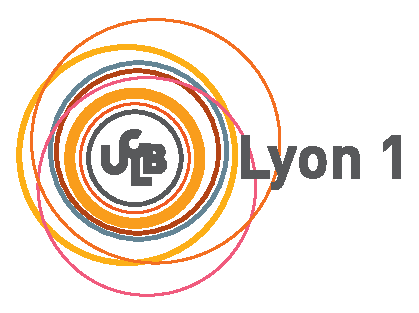
\includegraphics[height=2cm]{logoucbl.eps} \hfill 
\includegraphics[height=2cm]{logounivlyon.eps}

\vspace{0.5cm}

\begin{tabularx}{\textwidth}{@{} l X l @{} }
{\sc Licence Science de la matière} 	&	& Stage 2022--2023 \\
{\it \'Ecole Normale Sup\'erieure de Lyon}		&	&  \\
{\it Universit\'e Claude Bernard Lyon I}		& 	& L3 Physique
\end{tabularx}

\begin{center}

\vspace{1.5cm}

\rule[11pt]{5cm}{0.5pt}

\textbf{\huge Génération de seconde harmonique}

\rule{5cm}{0.5pt}

\vspace{1.5cm}

\parbox{15cm}{\small
	\textbf{R\'esum\'e}: \it L'équipe de Jérôme Beugnon du groupe Gaz quantiques du Laboratoire Kastler Brossel et du Collège de France, dirigé par Jean Dalibard, manipule des gaz de Bose 2D de rubidium. Le refroidissement et le piègeage des atomes nécessite de nombreux lasers, aux longeurs d'onde adaptées aux différentes transitions atomiques que l'on cherche à exploiter.
 %Les expériences de gaz d'atomes froids utilisent des lasers pour piéger les atomes qui doivent être à des longeurs d'ondes adaptées aux différentes transitions atomiques que l'on cherche à exploiter.
	L'objectif principal de mon stage a été la conception d'un laser à $\SI{532}{\nano\metre}$ (dans le vert) par génération de fréquence double à partir d'un laser infrarouge à 1064 nm. J'ai réalisé l'intégralité du montage et fait varier les différents paramètres disponibles afin d'essayer d'optimiser la puissance et la stabilité du faisceau vert produit. On constate que, du fait des effets thermiques, il est très difficile d'obtenir une puissance stable de l'ordre de quelques watts comme espéré. 
\vspace{0.5cm}
} 


\vspace{0.5cm}

\parbox{15cm}{
\textbf{Mots clefs} : \it optique non-linéaire, génération de seconde harmonique (SHG), niobate de lithium périodiquement polé (PPLN), fibre optique, cristaux photoniques}%TODO

\vspace{0.5cm}

\parbox{15cm}{
Stage encadr\'e par :

{\bf Jérôme \textsc{Beugnon}}

\href{mailto:beugnon@lkb.ens.fr}{\tt beugnon@lkb.ens.fr} / t\'el. (+33) 1 44 27 14 31


Laboratoire Kastler Brossel

{\it Adresse

Postale}

\url{http://adresse.web.du/laboratoire/}
} 

\vspace{0.5cm}


\includegraphics[height=5cm]{./img/logos.png}

%{\tiny \it Logos du laboratoire, de l'universit\'e d'accueil,\\ de l'organisme\ldots (\'eventuellement)}
\end{center}

\vfill
\hfill \today

\end{@empty}

\newpage

\thispagestyle{empty}
\section*{Remerciements}

Je tiens à remercier toute l'équipe Gaz quantiques du Laboratoire Kastler Brossel et du Collège de France pour son accueil chaleureux et pour m'avoir fait découvrir le monde de la recherche de l'intérieur. Je remercie tout particulièrement Franco Rabec pour avoir pris le temps de m'expliquer tous les détails de l'expérience sur laquelle il travaille et Guillaume Brochier pour sa disponibilité, son aide et ses précieux conseils. Je remercie également Benjamin Huard pour m'avoir conseillé ce stage. Enfin, je remercie Jérôme Beugnon, mon maîre de stage, pour sa disponibilité, ses conseils et toutes les connaissances qu'il m'a transmises, ainsi que pour le temps qu'il m'a consacré pendant mon stage mais également en amont pour planifier mon stage et préparer tout le matériel nécessaire. 
\tableofcontents
\newpage


\setcounter{page}{1}


\setlength{\parindent}{16pt}

\section{Introduction}
%Parler du labo, omniprésence des lasers (ralentissement, piègeage, excitation)

%Objectif: lasers IR moins chers et plus robustes -> obtenir du vert par SHG

\subsection{Expériences de rubidium}

La réalisation d'expériences de physique quantique sur des atomes nécessite de pouvoir les refroidir jusqu'à des températures en-dessous du Kelvin et, souvent, de les piéger dans des potentiels contrôlés. Le refroidissement et le piégeage d'atomes neutres est réalisé avec différentes techniques, parfois combinées ou enchaînées, mais toutes reposant sur l'utilisation de lasers, ce qui explique leur importance cruciale dans ces expériences.

Dans le projet Rubidium du groupe Gaz quantiques (LKB - Collège de France), les atomes refroidis et piégés par une séquence de pièges magnéto-optiques (MOT), de pièges magnétiques et optiques et de refroidissements par évaporation, que nous ne discuterons pas ici, sont ensuite confinés dans un plan pour former un condensat 2D avec de l'ordre de $10^6$ atomes à \SI{200}{nK}. Comme expliqué dans la sous-section suivante, un laser vert (à \lmbd{532}) pousse les atomes de rubidium vers un minimum d'intensité. Ainsi, en faisant interférer deux faisceaux cohérents inclinés, on réalise une figure d'interférence constituée de franges planes, comme on peut le voir figure \ref{fig:accordeon} (les 2 faisceaux en question sont les faisceaux vert clair sur la figure), et on cherche à confiner les atomes dans un des minima. Il faut également empêcher les atomes de s'échapper par les côtés, ce pour quoi on les éclaire avec un nouveau faisceau vert (vertical sur la figure) dont le profil, réalisé avec un DMD (\textit{digital mirror device}) est en forme d'anneau, ce qui permet de réaliser une ``boîte'' circulaire avec un puits de potentiel plat. Pour geler le degré de liberté vertical et obtenir un condensat 2D, on commence par piéger l'intégralité des atomes dans un même minimum d'intensité en créant une figure avec une interfrange large, puis on resserre progressivement l'interfrange en faisant varier l'inclinaison des faiceaux. En forçant une évaporation optique, on ne garde que les atomes moins énergétiques de sorte qu'à la fin l'intégralité des atomes soit dans le mode fondamental du puits. Le nuage d'atomes a alors une distribution gaussienne d'épaisseur de l'ordre de \lmbd{180} \citep{brice}. On voit figure \ref{fig:accordeon} en bleu une image des atomes piégés dans le cercle. Un deuxième DMD avec un nouveau laser vert peuvent alors être utilisés pour façonner différents potentiels à l'intérieur de la ``boîte''.

\begin{figure}[htbp]
	\centering
	%
	\begin{subfigure}[b]{0.48\textwidth}
    	\centering
    	\small
	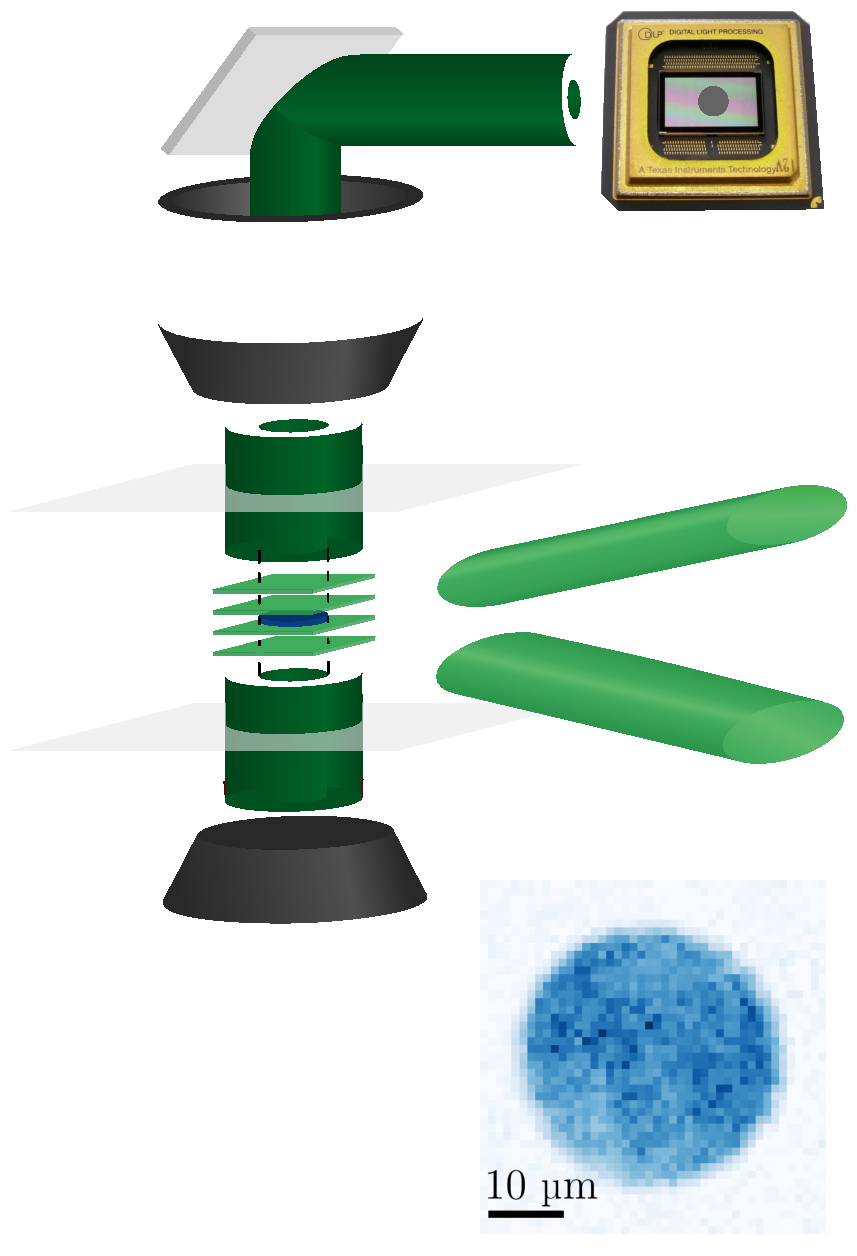
\includegraphics[height=9cm]{img/accordeon-dmd.pdf}
	\caption{\small Réalisation d'un piège circulaire 2D \footnotemark}
		\label{fig:accordeon}
	\end{subfigure}	
	%
	\begin{subfigure}[b]{0.48\textwidth}
		\centering
		\small
		\resizebox{!}{9cm}{
   			\begin{tikzpicture}[
level/.style = {
        ultra thick,
        red,
    },
    laser/.style = {
        ultra thick,
        green,
        dashed
    },
    connect/.style = {
        dashed,
        red
    },
    trans/.style={thick,->,shorten >=2pt,shorten <=2pt,>=stealth},
    notice/.style = {
        draw,
        rectangle callout,
        callout relative pointer={#1}
    },
    label/.style = {
        text width=2cm
    }
]
    % Draw all levels
    \draw[level] (0,0) --  +(-2,0) node[left] {$3S^{1/2}$} ;
    \draw[level] (0,4) --  +(-2,0) node[left] {$3P^{1/2}$} ;
    \draw[level] (0,4.5) --  +(-2,0) node[left] {$3P^{3/2}$};
    \draw[laser] (0,6) --  +(-2,0) node[left] {laser};
    
    \draw[trans] (-1.1,0) -- +(0,4) node[pos=0.4,left] {794.8 nm}; %794.8
    \draw[trans] (-1,0) -- +(0,4.5) node[pos=0.6,left] {780.0 nm}; %780.0
    \draw[trans] (-0.5,0) -- +(0,6) node[pos=0.85,left] {532 nm};
    
\end{tikzpicture}

		}
		\caption{\small Transitions du rubidium 87}
		\label{fig:transitions}
	\end{subfigure}
	%

	\caption{\small Utilisation du laser à \lmbd{532} dans l'expérience}
\end{figure}

\footnotetext{schéma réalisé par Brice Bakkali-Hassani, ancien doctorant sur l'expérience}


\subsection{Utilisation des lasers à 532 nm}

L'utilisations des lasers verts repose sur le principe du piégeage optique dipolaire, qui exploite l'interaction champ électrique-dipôle électrique induit. 
Cette interaction donne lieu, classiquement, à une force dérivant du potentiel $U_\mathsc{dip}(\v r) = -\frac12 \langle \v d \cdot \v E \rangle$=$-\frac{1}{2\varepsilon_0 c}\mathfrak{Re}\left(\alpha(\omega)\right) I(\v r)$ ($\v d$ désigne le moment dipolaire induit, $\alpha$ la polarisabilité complexe, $\langle \cdot \rangle$ une moynne temporelle et $I$ l'intensité du faisceau)
%\footnote{Le facteur $\frac12$ est dû au fait que le dipôle est non pas permannent mais proportionnel au champ appliqué.} %En effet, pour $\v d = \alpha \v E$, $\v F = (\v d \cdot \v \nabla) \v E = \frac12 \v \nabla (\v d \cdot \v E)$}  %
qui va servir à piéger les atomes dans un minimum de potentiel. Le piégeage est perturbé par les cycles d'absorption et réémission spontanée, ayant lieu, toujours ``classiquement'', à une fréquence $\Gamma_\mathsc{diff} = \frac{P_\mathsc{abs}}{\hbar \omega} = \frac{1}{\hbar \varepsilon_0 c} \mathfrak{Im}\left(\alpha(\omega)\right) I(\v r)$ où $P_\mathsc{abs} = \langle \dot{\v d} \cdot \v E \rangle$ est la puissance absorbée par l'atome. 
Pour un atome à deux niveaux avec une transition à $\omega_0$, dans l'approximation de faible saturation (état excité faiblement peuplé) et de fort désaccord ($\Delta = \omega - \omega_0$ vérifiant $|\Delta| \ll \omega_0$), vérifiée en pratique et permettant de justifier le calcul classique (à une précision de l'ordre du pourcent), on trouve

\begin{salign}
	U_\mathsc{dip}(\v r)=\frac{3\pi c^2}{2\omega_0^3} & \frac{\Gamma}{\Delta} I(\v r) \\
	\Gamma_\mathsc{diff}(\v r)=\frac{3\pi c^2}{2\hbar\omega_0^3} & \left(\frac{\Gamma}{\Delta}\right)^2 I(\v r) \\
\end{salign}

avec $\Gamma = \frac{\e 2 \omega^2}{6 \pi \varepsilon_0 m_e c^3}$ le facteur d'amortissement dû au rayonnement.

Puisque $\Gamma_\mathsc{diff}=\frac{\Gamma}{\hbar \Delta} U_\mathsc{dip}$, on voit qu'un grand désaccord permet de minimiser l'effet perturbateur de la diffusion. On remarque également que pour un faisceau laser désaccordé vers le rouge, l'atome est piégé dans les zones lumineuses, alors que pour un désaccord vers le bleu (comme c'est le cas pour le rubidium et le laser vert), l'atome est piégé dans les zones sombres.

Pour un atome réel à plusieurs niveaux, l'énergie d'interaction (qui s'obtient plus rigoureusement en considérant la perturbation par un hamiltonien de couplage $\mathcal H_1 = - \hat{\v d} \cdot \v E$ des états propres du système atome + champ) est la somme des contributions des différents états excités, pondérée par l'importance des transitions associées \citep{grimm}. Pour les atomes de rubidium 87 utilisés dans l'expérience, les transitions prépondérantes sont les 2 transitions de la ligne D, pour lesquelles le laser vert à $\SI{532}{\nano\metre}$ est désaccordé vers le bleu (figure \ref{fig:transitions})


\subsection{Objectif du stage}

Les lasers verts actuellement utilisés au laboratoire sont des lasers à \lmbd{1064} Nd-Yag ou à diode avec amplificateur à semi-conducteur (\textit{tapered amplifier}) qui sont vendus directement avec le doublage de fréquence. Ils ont l'inconvénient d'être particulièrement onéreux et fragiles, et leur réparation nécessite plusieurs mois d'attente. L'objectif de mon projet était donc d'explorer la possibilité de réaliser le doublage soi-même à partir d'un laser à \lmbd{1064} beaucoup plus facile d'accès. Ce doublage de fréquence (SHG pour \textit{second harmonic generation} en anglais) repose sur l'existence d'un terme dans la polarisation électrique de certains cristaux quadratique en le champ appliqué, qui joue le rôle d'un terme source à la fréquence double de celle du faisceau incident. C'est notamment le cas du niobate de lithium choisi par mon maître de stage, Jérôme Beugnon, pour ce projet. %Le principe sera expliqué plus en détail section \ref{SHG}. 

\section{Couplage de la fibre à cristaux/al? photoniques}
Une première partie de mon stage, indépendante de l'objectif principal d'obtenir un laser vert, a été de tester une fibre à cristaux photoniques
%, plus précisément une fibre de verre à trous (\textit{holey fiber}) 
LMA-PM-10 de la marque NKT Photonics. LMA signifie large (effective) mode area et donc que la fibre est faite pour des faisceaux larges, ce qui est important pour les applications avec des lasers de plusieurs dizaines de watts, car le seuil de destruction des matériaux ainsi que les effets thermiques dus à la dissipation dépendent de l'intensité et non de la puissance totale.
La technologie des fibres optiques traditionnelles, reposant sur une réflexion interne totale, ne permet pas de fabriquer des fibres à c\oe ur large qui resteraient monomodes sur une gamme de longueurs d'ondes et de rayon de courbure de la fibre suffisante. 
Les fibres à cristaux photoniques, quant à elles, reposent sur une variation d'indice optique effectif périodique grâce à une structure régulière de trous et ont l'avantage de permettre beaucoup plus de liberté, notamment en terme de taille du c\oe ur tout en restant monomodes, et ce sur une très large gamme de fréquences.  
%Cette structure conduit à des bandes interdites analogues à celles des électrons dans un crystal (ondes de Bloch). 
\citep{russell2006,russell2007}

%Contrairement aux fibres traditionnelles, la variation d'indice optique dans ces fibres est réalisée à l'aide d'une structure régulière de trous. En effet, l'air aillant un indice optique inférieur au matériau de la fibre, les trous permettent de réduire l'indice moyen. % TODO: corriger

\begin{figure}[htpb] 
\centering
\hspace*{0.4cm}
\begin{subfigure}[h]{0.48\textwidth}
	\centering
	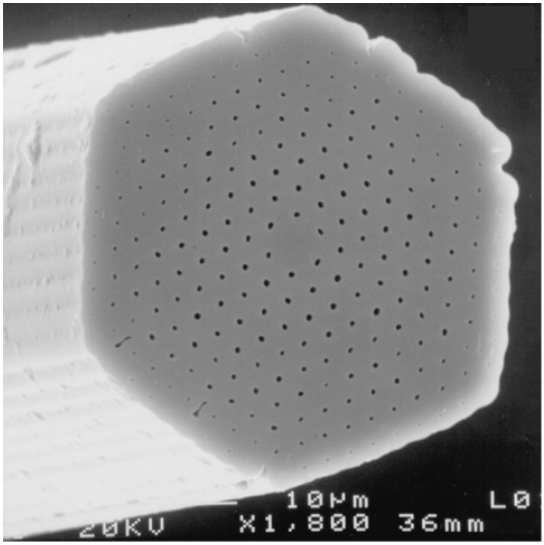
\includegraphics[height=5cm]{../biblio/solid core PCF - russell2006}
	\caption{Image par microscopie électronique par balayage de la première fibre à cristaux photoniques fonctionnelle \ncite{russell2006}}
	\label{fig:PCF}
\end{subfigure}
%\hspace*{0.4cm}
\begin{subfigure}[h]{0.48\textwidth}
	\centering
	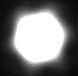
\includegraphics[height=5cm]{./img/mode hexa.png}
	\caption{Image en intensité du mode hexagonal en sortie (caméra fortement saturée)}
	\label{fig:hexa}
\end{subfigure}
\hspace*{-0.8cm}
\caption{Structure de la fibre à cristaux photoniques et mode hexanogal en sortie}
\end{figure}

Comme indiqué, la fibre à cristaux photoniques ne sélectionne qu'un seul mode. Les fibres monomodes traditionnelles sélectionnent généralement un mode gaussien, mais la géométrie de la fibre à cristaux photoniques utilisée fait que le mode sélectionné est un mode hexagonal, comme on peut le voir figure \ref{fig:hexa}. Ce mode ne se distingue cependant que très peu d'un mode gaussien, et on ne voit la forme hexagonale qu'en saturant la caméra.

En particulier, afin de maximiser la transmission de la fibre, il faut que l'axe du faisceau incident (gaussien) coïncide avec celui de la fibre, ce qui correspond à l'ajustement de 4 paramètres (2 angles pour l'orientations et 2 coordonnées pour la position dans le plan transverse). L'ajustement est fait à l'aide de 2 miroirs (cf schéma figure \ref{fig:couplage}). Il faut également que le faisceau ait le bon waist et qu'il soit focalisé en bout de fibre. La focalisation est réalisée à l'aide d'un coupleur de fibre (60SMS-SMA-0-M5-08 de la marque Schäfter+Kirchhoff), qui est un collimateur de focale 5 mm optimisé pour le couplage de fibres et nécessite de produire un faisceau collimaté au niveau du coupleur avec le bon waist (que l'on peut déterminer expérimentalement en observant le faisceau en sortie de fibre, puisqu'elle est équipée d'un coupleur identique). Cet ajustement est fait à l'aide d'un téléscope avec des focales adaptées.

\begin{figure}[h]
	\centering
	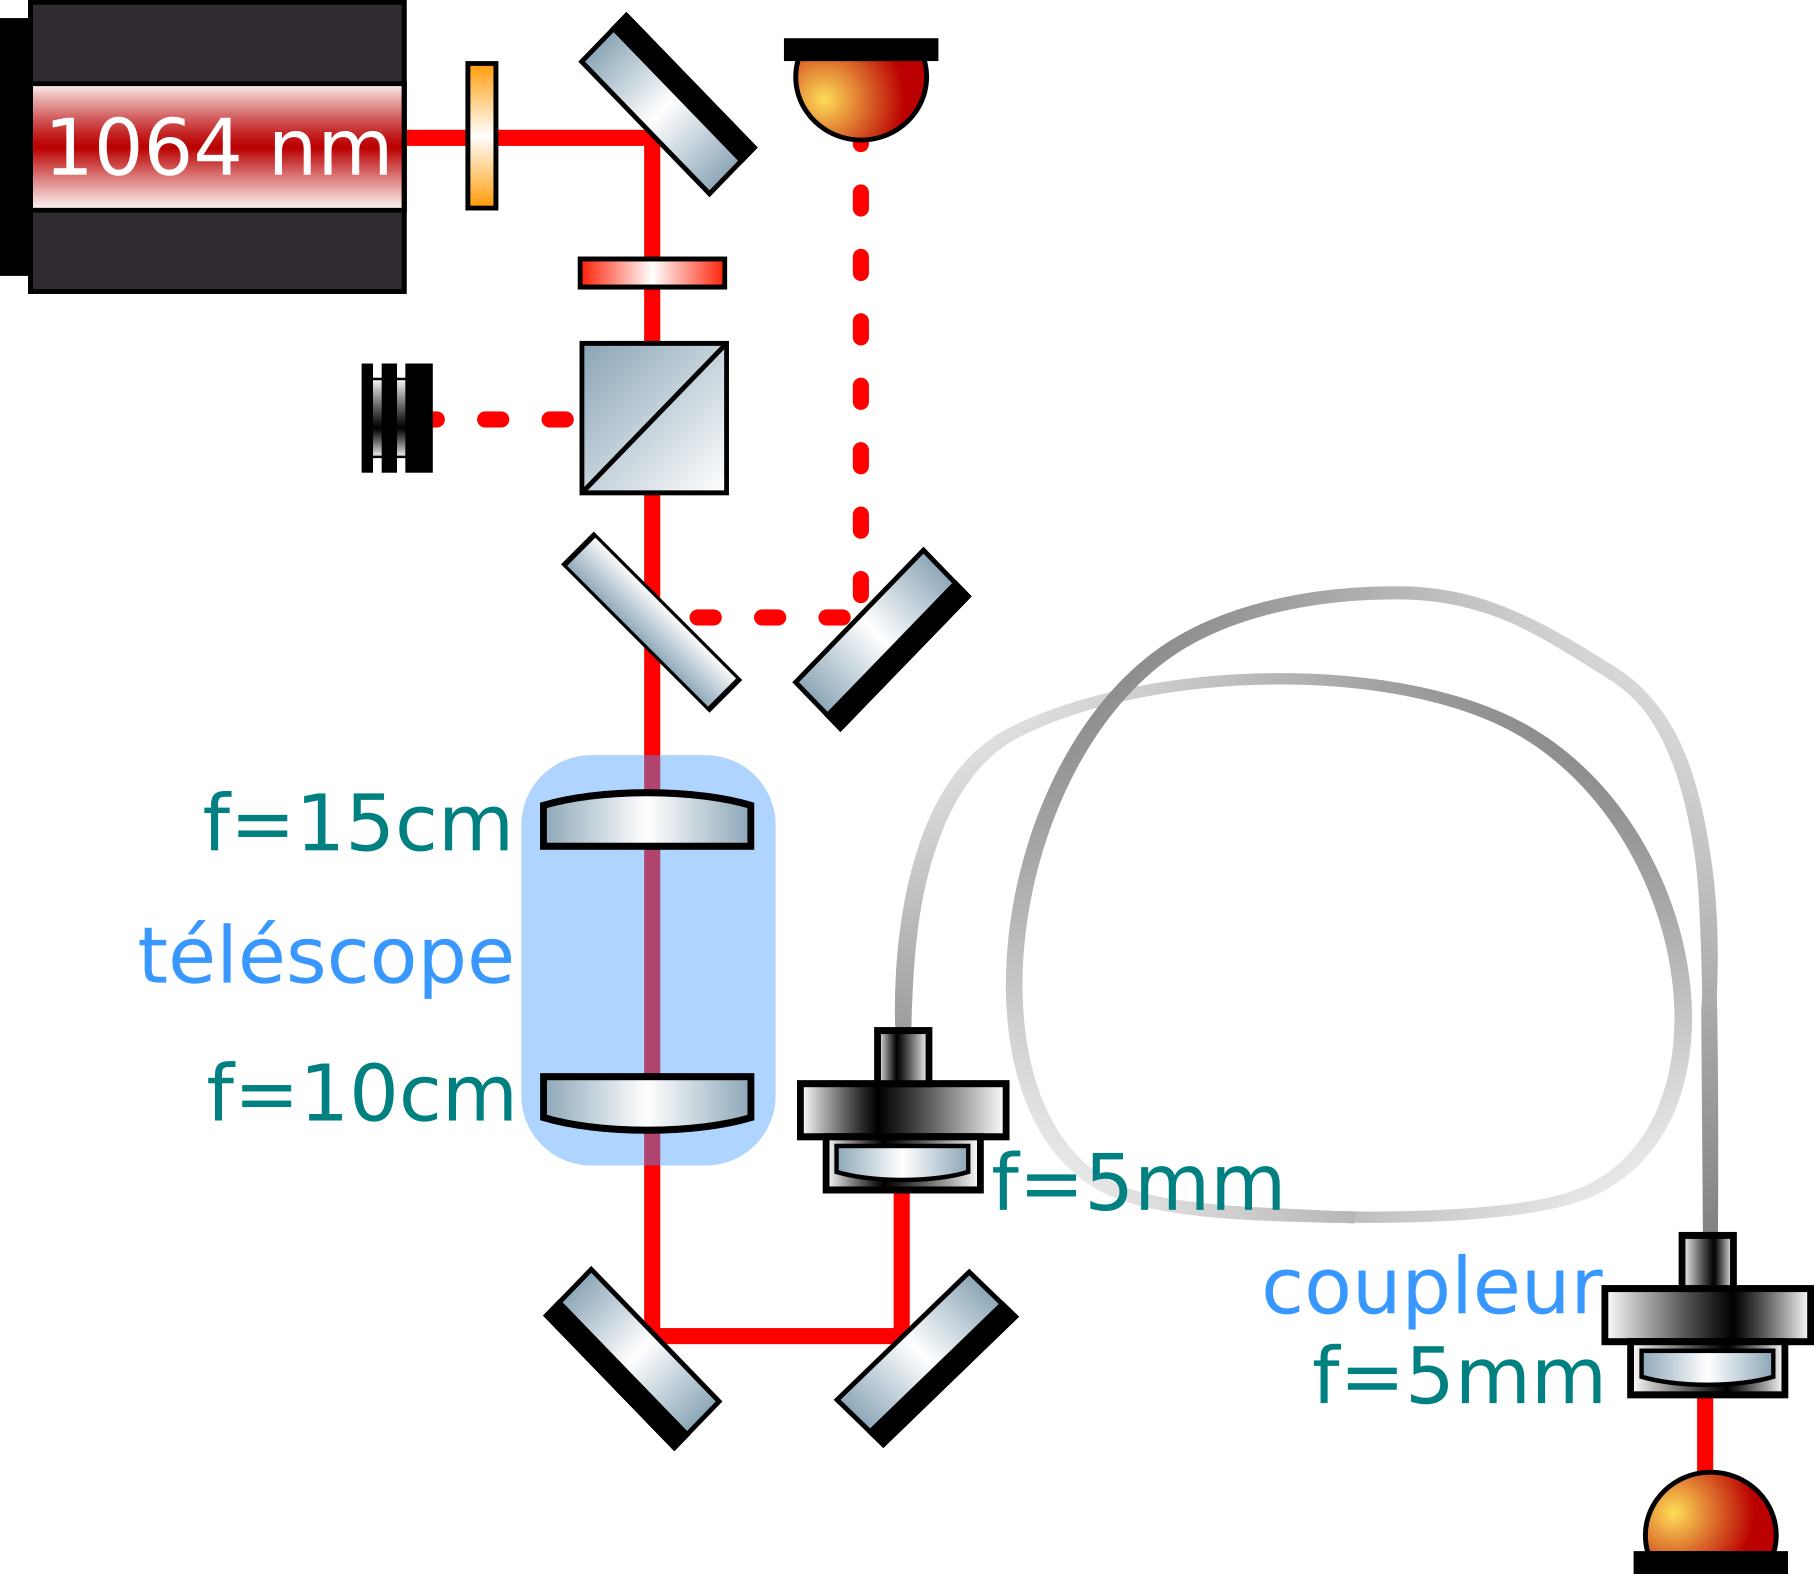
\includegraphics[width=0.7\textwidth]{./img/schema couplage.png}
	\caption{Montage de la fibre à cristaux photoniques}
	\label{fig:couplage}
\end{figure}

TODO: injection en pola


\section{Principe de la génération de seconde harmonique (SHG)} %\'Etude th\'eoriqaue de la génération de seconde harmonique (SHG)}
\label{SHG}

Nous revenons maintenant à l'objectif principal du stage, l'obtention d'un laser à \lmbd{532} par génération de seconde harmonique, dont nous expliquons d'abord le principe.

\subsection{Polarisation non linéaire et seconde harmonique}

\begin{figure}[h]
\centering
\begin{subfigure}{0.45\textwidth}
	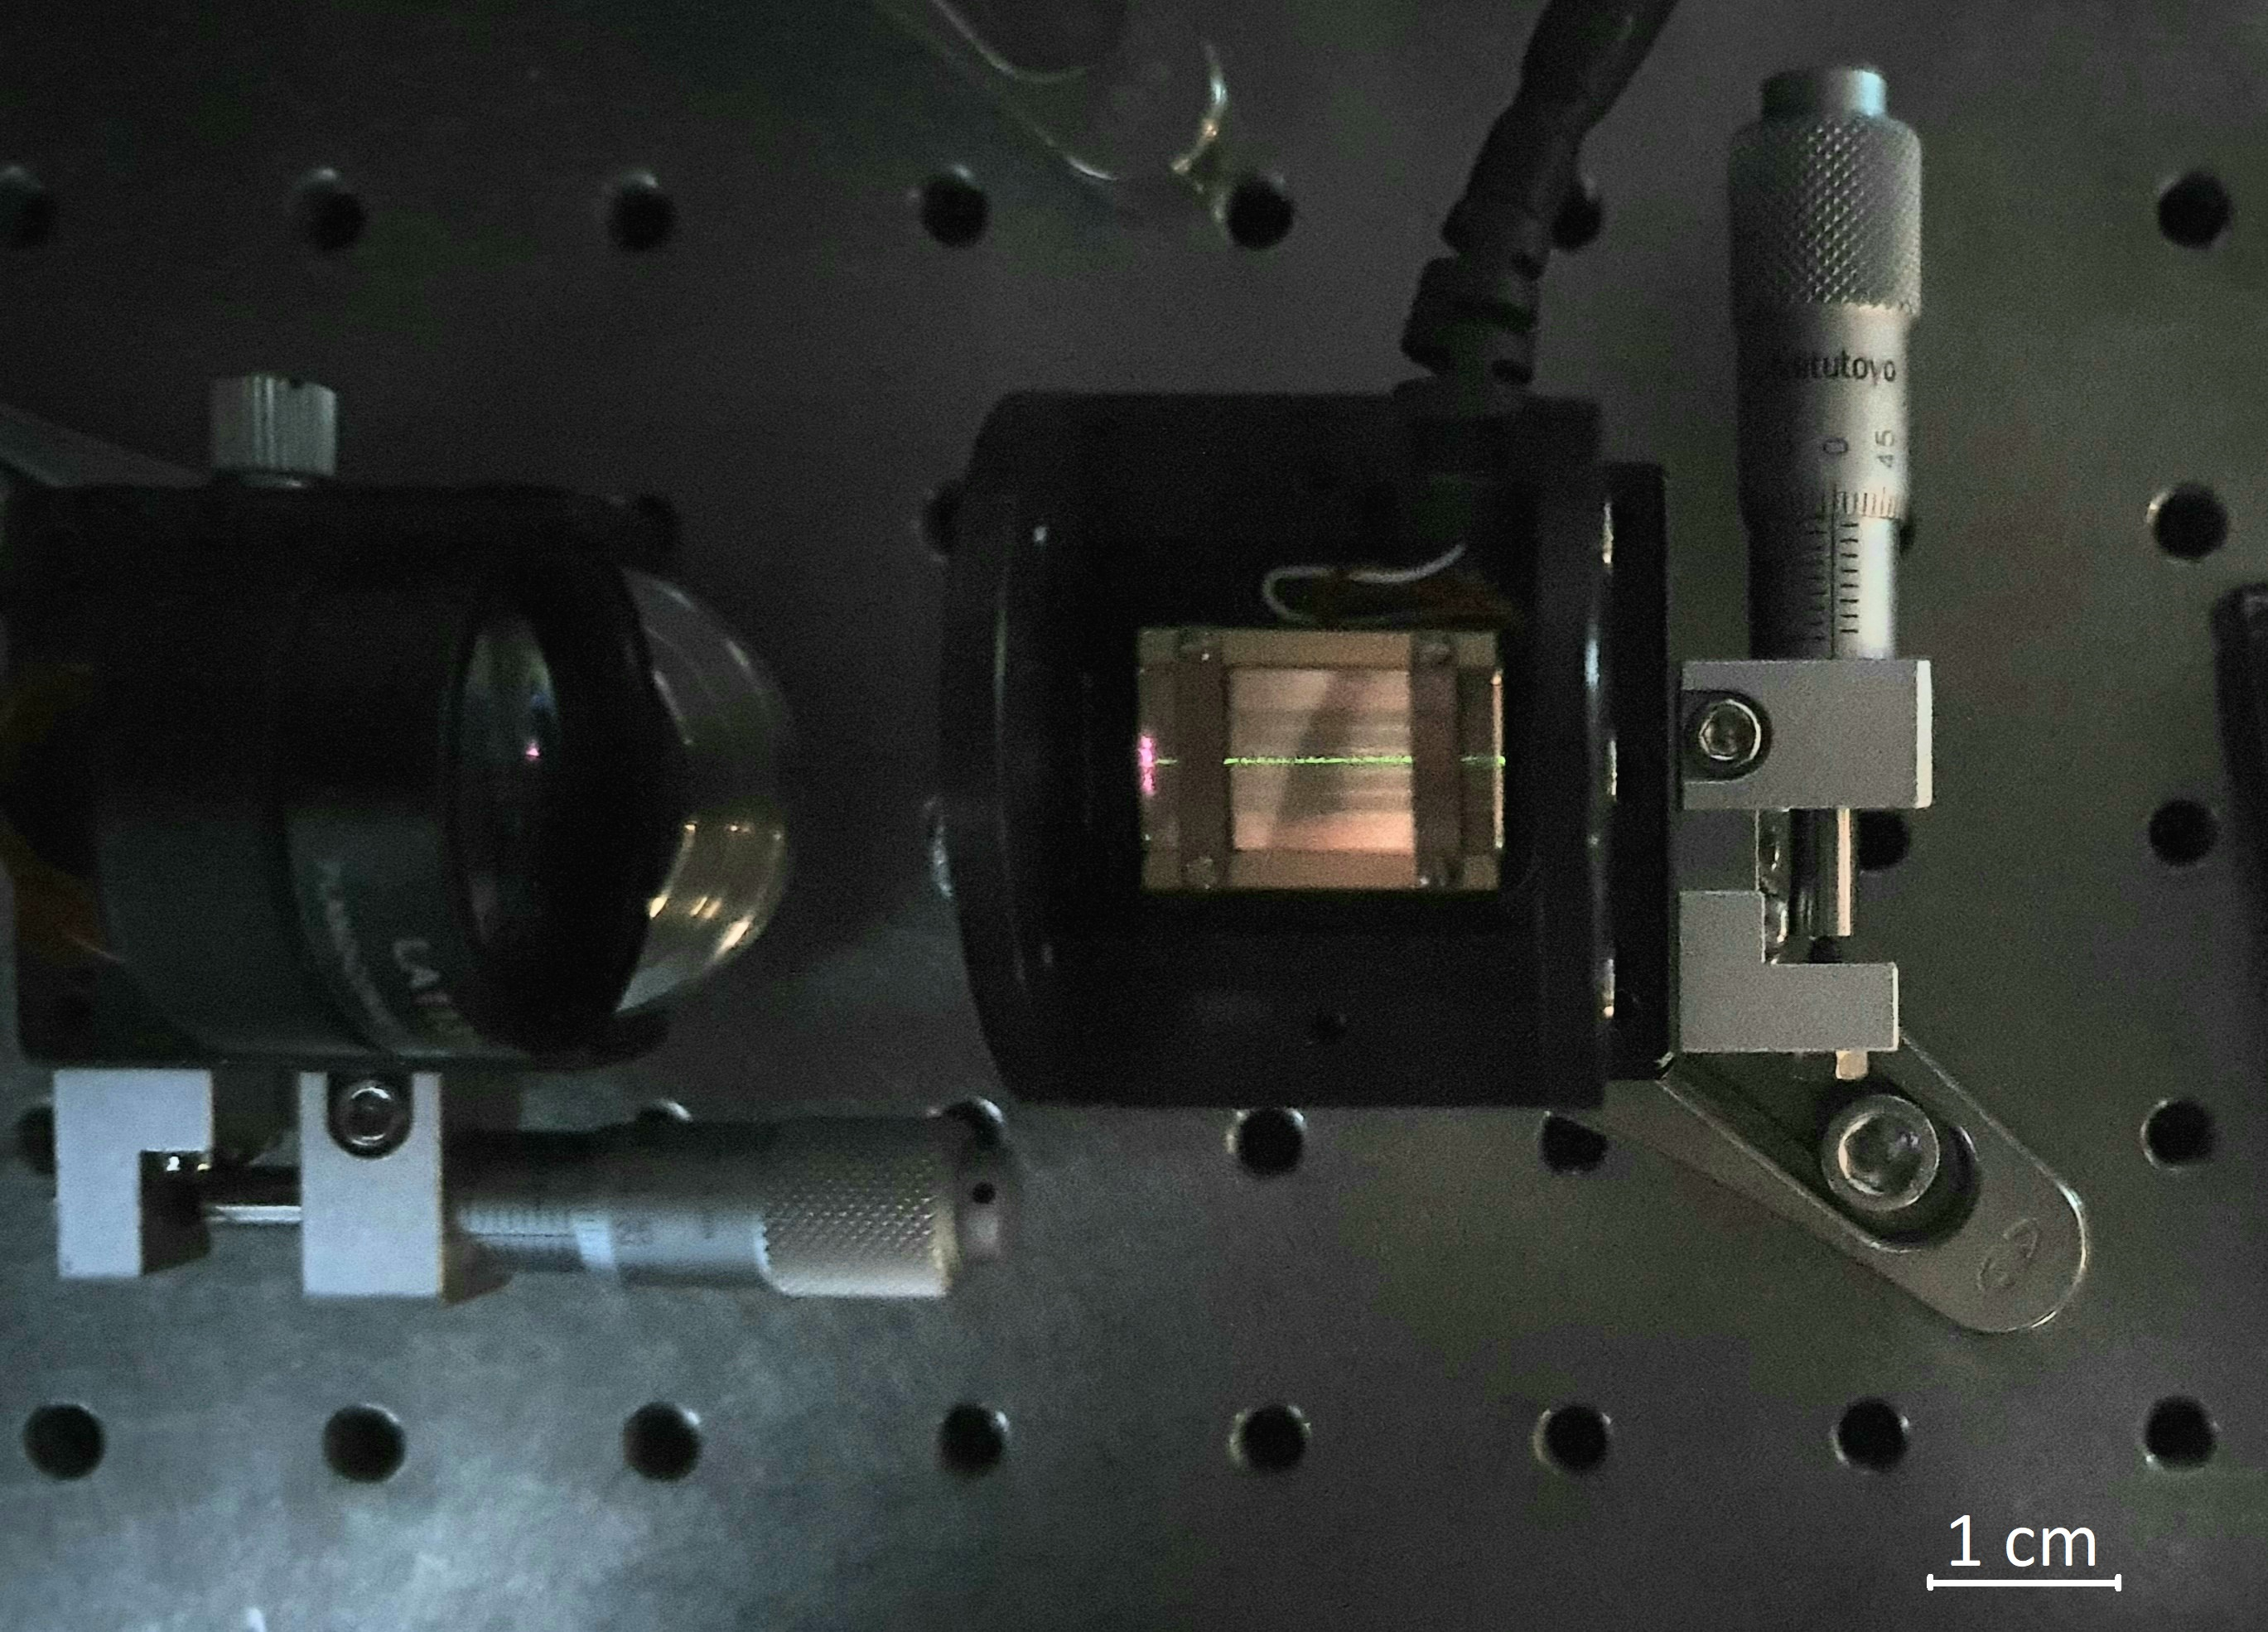
\includegraphics[width=\textwidth]{./img/cristal clair.jpg}
\end{subfigure}
\begin{subfigure}{0.5\textwidth}
	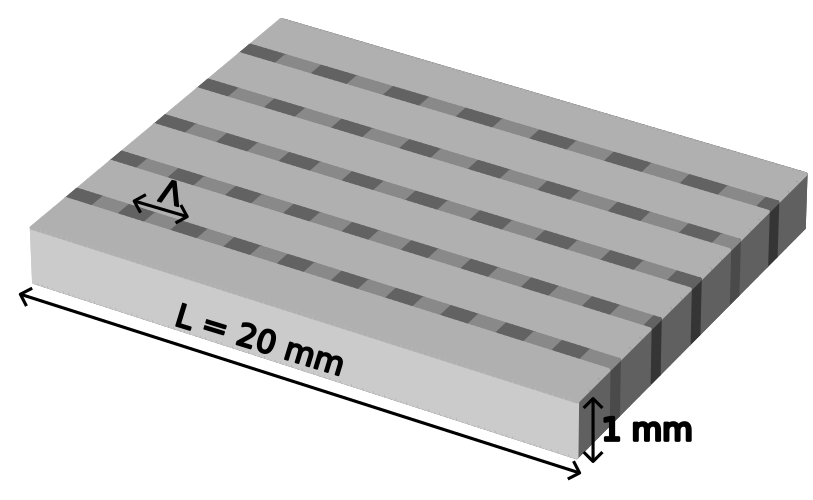
\includegraphics[width=\textwidth]{./img/cristal.png}
\end{subfigure}
\caption{Génération d'un laser vert dans un cristal doubleur de fréquence}
\label{fig:cristal}
\end{figure}

La génération de la seconde harmonique a lieu dans un cristal doubleur de fréquence avec des propriétés non-linéaires favorables (figure \ref{fig:cristal}).
La propagation d'ondes électromagnétiques dans un milieu non linéaire donne lieu à une équation d'onde avec un terme source, qui s'écrit (cf annexe \ref{NL}) \ncite{boyd,joffre}
\[ \nabla^2 \v E_q(\v r) + \frac{\omega_q^2}{c^2}\tens\epsilon^{(1)}(\omega_q)\cdot \v E_q(\v r) = - \frac{\omega_q^2}{\epsilon_0 c^2} \v P^\mathsc{NL}_q(\v r) \]
dans le domaine de Fourier en temps avec la convention $\v E(\v r, t) = \mathfrak{Re} \left\{ \sum_{n \in \mathbb Z} \v {\boldsymbol{\mathcal E}}_q (\v r) \e{-i q \omega t} \right\}$,
%, avec n un indice désignant la composante spectrale (il s'agira dans notre cas de l'ordre de l'harmonique), 
avec $\tens \epsilon^{(1)}$ le tenseur de permittivité diélectrique relative associé à la partie linéaire de la polarisation et $\v P^\mathsc{NL}_q$ la partie non-linéaire de la polarisation.

On fait l'hypothèse simplificatrice d'une polarisation linéaire selon un des axes principaux et on travaillera par la suite avec des $\mathcal E_q$ scalaires. En particulier, la permittivité tensorielle $\tens \varepsilon^{(1)}$ est remplacée par sa valeur propre correspondante et donne lieu à un indice optique $n_q^2 = 1 + \varepsilon^{(1)}(\omega)/\varepsilon_0$. En écrivant les différentes harmoniques sous la forme d'une ``onde monochromatique d'amplitude variable'' $\mathcal E_q = \A_q(x,y,z) \e{ik_qz}$ avec $\boxed{k_q =\frac{n_q \omega_q}{c}}$ et en se plaçant dans l'approximation paraxiale, i.e. de lente variation de $\A$ avec $z$ $\left(\frac{\partial^2 \A_q}{\partial z^2} \ll k_q \frac{\partial \A_q}{\partial z}\right)$, on arrive aux équations \ncite{joffre}
\begin{align*}  
	\left\{\v\nabla_\bot + 2 i k_q \frac{\partial}{\partial z} \right\} \A_q =
\end{align*}
avec $\v\nabla_\bot = \pdv{}{x^2} + \pdv{}{y^2}$.

En particulier, pour un champ électrique avec une composante à $\omega$ et une à $2\omega$, le terme quadratique dans la polarisation est donné par \ncite{joffre}
\begin{align*}
	P^{(2)} &= \varepsilon_0 \chi^{(2)} \v E^2  \text{ avec $\chi^{(2)}$ la susceptibilité d'odre 2}\\
	&= \frac{\varepsilon_0 \chi^{(2)}}{4} \left\{\mathcal E_1 e^{-i\omega t} + \mathcal E_1^*i e^{i\omega t} + \mathcal E_2 e^{-2i\omega t} + \mathcal E_2^* e^{2i\omega t} \vphantom{\frac12}\right\}^2 \\
	&= \frac{\varepsilon_0 \chi^{(2)}}{4} \left\{\mathcal E_1^2 \e{-2i\omega t} + \E_1^{*2} \e{2i\omega t} + 2|\mathcal E_1|^2 + 2 \E_1\E_2^* \e{i\omega t} + 2 \E_1^*\E_2 \e{-i\omega t} \vphantom{\frac12}\right. \\
	&\qquad\qquad\qquad \left. + 2 \E_1\E_2 \e{-3 i\omega t}  + 2 \E_1^*\E_2^* \e{3 i\omega t} + \mathcal O(\E_2^2) \vphantom{\frac12}\right\}
\end{align*}
où l'on a considéré que $\chi^{(2)}$ est le même pour toutes les harmoniqes pour un milieu supposé sans pertes \ncite{boyd}.

On voit donc que l'onde incidente (à $\omega$) conduit à un terme à la fréquence double dans la polarisation, qui va conduire à la création d'une onde à cette seconde harmonique comme souhaité. Cette dernière va conduire à un terme à la fréquence fondamentale qui va affecter l'onde incidente ainsi qu'à un terme à la fréquence triple qui va conduire à une onde à la troisième harmonique et ainsi de suite. 
Dans l'hypothèse où la seconde harmonique est d'amplitude faible par rapport au faisceau incident, nous pouvons cependant négliger ces termes d'ordre supérieur. Cette hypothèse, connue sous le nom \textbf{d'hypothèse de non-déplétion}, est discutée en annexe \ref{ndepl}. Nous négligerons également le terme constant dit de redressement. %Nous nous plaçons cependant dans l'hypothèse que la seconde harmonique 

%En écrivant les différents champs 

%Plus précisément, en écrivant les équations d'onde paraxiales pour les différentes harmoniques, 

Ceci conduit à l'équation d'évolution de l'amplitude de l'onde générée $\A_2$ suivante:
\[ \left\{\v\nabla_\bot + 2 i k_2 \frac{\partial}{\partial z} \right\} \A_2 = - \frac{2 \chi^{(2)} \omega^2}{c^2} \A_1^2 \e{- i (k_2 - 2k_1) z} \]

\subsection{Le problème de l'accord de phase}

Cette équation est beaucoup plus abordable dans l'approximation d'une onde plane avec $\A_1$ et $\A_2$ ne dépendant que de $z$ (et donc $\A_1$ constante dans \textbf{l'hypothèse de non-déplétion}):
\begin{align}
	\dv{\A_2}{z} &= i\frac{\chi^{(2)}\omega}{2cn_2} \A_1^2 \e{-i \Delta k z} \text{ avec } \boxed{\Delta k = k_2 - 2k_1} \label{eq:pwe} \\
	\text{soit } \A_2(L) &= i \frac{\chi^{(2)}\omega}{2 cn_2} \A_1^2 L \operatorname{sinc}\left( \frac{\Delta k L}{2} \right) \e{-i\frac{\Delta k L}{2}}
\end{align}
en sortie du cristal en $z=L$ avec $\A_2(0)=0$ à l'entrée.

Cette équation se comprend très bien en considérant que le carré de l'onde incidente, de nombre d'onde $2k_1$, génère un rayonnement qui se déplace ensuite à $k_2$, de sorte qu'en un point $z$ une onde de phase $2k_1z$ vient s'ajouter à une onde se propageant à $k_2$. Ainsi, l'onde à la seconde harmonique générée en $z$ aura à la sortie du cristal en $z=L$ la phase $2k_1 z + k_2 (L-z) = k_2 L - \Delta k z$ (modulo une constante universelle), de sorte que les ondes générées en $z$ et en $z+L_\mathsc{coh} =z + \frac{\pi}{\Delta k}$ interfèrent destructivement, ce qui conduit à une amplitude nulle en sortie, comme illustré figure \ref{fig:agen}.

\begin{figure}[htpb]
\centering
\begin{subfigure}[h]{0.48\textwidth}
	\centering
	\hspace*{-0.8cm}
	%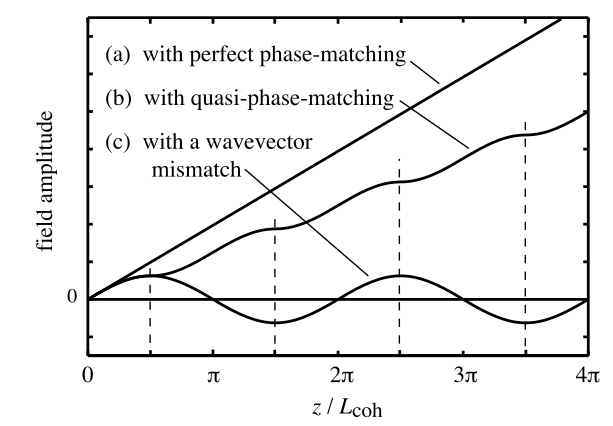
\includegraphics[height=5cm]{./img/QPM.png}
	\include{./img/qpm.tex}
	\caption{}
	\label{fig:agen}
\end{subfigure}
\begin{subfigure}[h]{0.48\textwidth}
	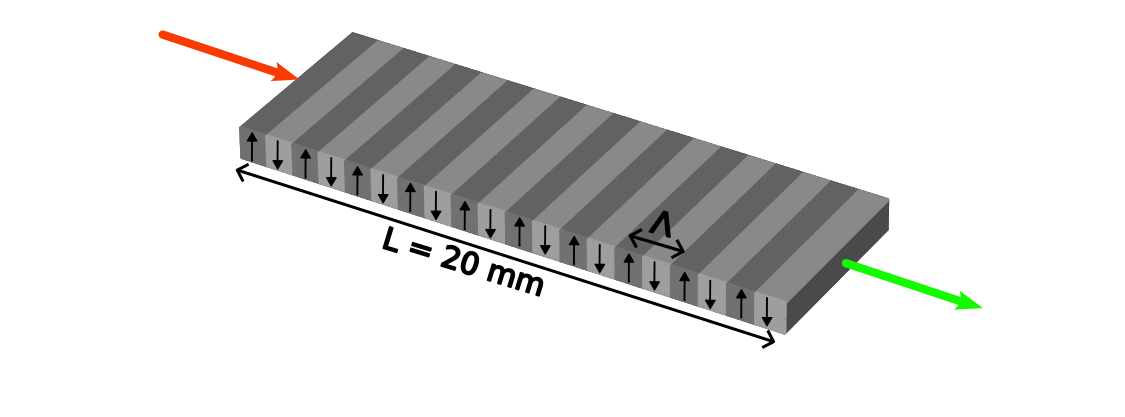
\includegraphics[height=4cm]{./img/PP.png}
	\caption{}
\end{subfigure}
\hspace*{-0.6cm}
\caption{Amplitude de seconde harmonique et quasi-accord de phase} %TODO
\label{fig:QPM}
\end{figure}

Avec le cristal de niobate de lithium utilisé, $L_\mathsc{coh}$ vaut à peine $\SI{3}{\micro\meter}$ alors que le cristal fait $\SI{2}{cm}$.
Afin d'avoir une génération efficace, il faudrait donc $\Delta k = \frac{2\pi}{\lambda_2}(n_2-n_1) = 0$ (condition d'accord de phase) avec $\lambda_2=$\lmbd{532} la longueur d'onde dans le vide de la seconde harmonqiue, soit $n_2 = n_1$. Cela n'est \textit{a priori} pas possible sans dispersion anormale. Une solution consiste alors à exploiter la biréfringence du cristal, mais cette méthode est difficile à réaliser et le $\chi^{(2)}$ correspondant à la polarisation requise est souvent assez faible. 

Nous avons choisi une autre solution qui consiste à fabriquer un cristal dont le $\chi^{(2)}$ varie spatialement. En effet, si $\chi^{(2)}(z) = \chi^{(2)}_0 \e{i k_\chi z}$, cela revient à remplacer $\Delta k$ par $\Delta k_\mathsc{eff} = \Delta k - k_\chi$ dans (\ref{eq:pwe}). En pratique, il est difficile de fabriquer un tel cristal, et on préfère inverser le signe de $\chi^{(2)}$ en inversant l'axe extraordinaire d'un matériau ferroélectrique avec une période $\Lambda$ (cf figure \ref{fig:QPM}). On parle alors de quasi-accord de phase et un tel cristal est dit périodiquement pôlé. Dans ce cas, la décomposition de Fourier de $\chi^{(2)}(z) = \chi^{(2)}_0 \operatorname{sgn}[\cos(2\pi z/ \Lambda)]$ montre que le terme de plus grande amplitude est le fondamental d'amplitude $\chi_\mathsc{eff} = \frac2\pi \chi^{(2)}_0$ et de nombre d'onde $k_\chi = \frac{2\pi}{\Lambda}$. Si $k_\chi = \Delta k$, le terme source correspondant sera accordé en phase sur toute la longueur du cristal et permettra donc de générer la seconde harmonique. Par la suite, on ne tiendra compte que de ce terme, oubliant les autres harmoniques de $\chi^{(2)}(z)$.
Ceci nous conduit à une amplitude 
\begin{align}
	&\A_2(L) = i \frac{\chi_\mathsc{eff} \omega}{2 cn_2} \A_1^2L \\	
	\text{et } i &\frac{\chi_\mathsc{eff}\omega}{2 cn_2} \A_1^2 L \operatorname{sinc}\left( \frac{\Delta k_\mathsc{eff} L}{2} \right) 
	\e{-i\frac{\Delta k_\mathsc{eff} L}{2}}
\end{align}
si le quasi-accord de phase n'est pas respecté.

En termes de puissance, la puissance de la seconde harmonique est quadratique en la puissance du fondamental, avec une efficacité (normalisée)
\begin{align}
	\alpha &= \frac{\mathcal P_2}{\mathcal P_1^2} = \frac{\frac12 n_2 \varepsilon_0 c |\A_2|^2}{\left(\frac12 n_1 \varepsilon_0 c |\A_1|^2\right)^2} 
	= \frac{\chi_\mathsc{eff}^2\omega^2}{2 n_2 n_1^2 \varepsilon_0 c^3} L^2
\end{align}

On notera en particulier la dépendance quadratique en la longueur du cristal, qui serait perdue en l'absence d'accord de phase.

\subsection{Cas des faisceaux gaussiens}

En réalité, profil spatial, solution sans terme source: faisceau gaussien.

Mode q: source polarisation quadratique en l'amplitude du fondamental -> même profil transverse que $\v E_1^2 \propto \left( \e{-\left(\frac{r}{w(z)}\right)^2} \right)^2 = \e{-\left(\frac{r}{w(z)/ \sqrt 2}\right)^2}$ ce qui conduit à la supposition que le faisceau vert produit est ``gaussien'' (le profil transverse est gaussien mais la puissance varie longitudinalement) avec la même longueur de Rayleigh et un waist $\sqrt 2$ fois plus petit (ce qui est cohérent pour une longuer d'onde moitié).

On pose donc l'Ansatz suivant \[ A_2 = \frac{\mathcal A_2(z)}{1+i\zeta}\e{} \] qui correpond finalement à varier la constante dans la solution de l'équation linéaire (sans ``terme source'').

$\mathcal A_2$ vérifie alors l'équation d'évolution suivante

\dots

On obtient donc 
\begin{align}
	\alpha = 	
\end{align}

\begin{figure}[htpb] 
\centering
\hspace*{-0.8cm}
\begin{subfigure}[b]{0.48\textwidth}
	\small
	% This file was created with tikzplotlib v0.10.1.
\begin{tikzpicture}

\definecolor{darkgray158}{RGB}{158,158,158}
\definecolor{darkgray176}{RGB}{176,176,176}
\definecolor{darkorange2551490}{RGB}{255,149,0}
\definecolor{darkslategray71}{RGB}{71,71,71}
\definecolor{limegreen018569}{RGB}{0,185,69}
\definecolor{orangered255440}{RGB}{255,44,0}
\definecolor{slategray13291151}{RGB}{132,91,151}
\definecolor{teal1293165}{RGB}{12,93,165}

\begin{axis}[
legend cell align={left},
legend style={
  fill opacity=0.8,
  draw opacity=1,
  text opacity=1,
  at={(0.03,0.97)},
  anchor=north west,
  draw=none
},
tick pos=both,
x grid style={darkgray176},
xlabel={\(\displaystyle b\)},
xmin=-4.4, xmax=4.4,
xtick style={color=black},
xtick={-6,-4,-2,0,2,4,6},
xticklabels={
  \(\displaystyle {\ensuremath{-}6}\),
  \(\displaystyle {\ensuremath{-}4}\),
  \(\displaystyle {\ensuremath{-}2}\),
  \(\displaystyle {0}\),
  \(\displaystyle {2}\),
  \(\displaystyle {4}\),
  \(\displaystyle {6}\)
},
y grid style={darkgray176},
ylabel={\(\displaystyle h(a,b)\)},
ymin=-0.0533755941486969, ymax=1.12088747765006,
ytick style={color=black},
ytick={-0.2,0,0.2,0.4,0.6,0.8,1,1.2},
yticklabels={
  \(\displaystyle {\ensuremath{-}0.2}\),
  \(\displaystyle {0.0}\),
  \(\displaystyle {0.2}\),
  \(\displaystyle {0.4}\),
  \(\displaystyle {0.6}\),
  \(\displaystyle {0.8}\),
  \(\displaystyle {1.0}\),
  \(\displaystyle {1.2}\)
}
]
\addplot [very thick, teal1293165]
table {%
-4 0.0329347308512046
-3.97333333333333 0.0343055825245623
-3.94666666666667 0.0357080043590585
-3.92 0.0371420839779771
-3.89333333333333 0.038607898881193
-3.86666666666667 0.0401055163340945
-3.84 0.0416349932601001
-3.81333333333333 0.0431963761368276
-3.78666666666667 0.044789700895989
-3.76 0.0464149928270652
-3.73333333333333 0.0480722664848272
-3.70666666666667 0.0497615256007613
-3.68 0.051482762998457
-3.65333333333333 0.0532359605130127
-3.62666666666667 0.0550210889145177
-3.6 0.0568381078356582
-3.57333333333333 0.0586869657035041
-3.54666666666667 0.0605675996755226
-3.52 0.0624799355798691
-3.49333333333333 0.0644238878599992
-3.46666666666667 0.0663993595236489
-3.44 0.0684062420962228
-3.41333333333333 0.070444415578633
-3.38666666666667 0.0725137484096269
-3.36 0.07461409743264
-3.33333333333333 0.0767453078672096
-3.30666666666667 0.078907213284981
-3.28 0.0810996355903408
-3.25333333333333 0.0833223850056993
-3.22666666666667 0.0855752600614574
-3.2 0.0878580475906748
-3.17333333333333 0.0901705227284692
-3.14666666666667 0.092512448916163
-3.12 0.0948835779101949
-3.09333333333333 0.0972836497958193
-3.06666666666667 0.0997123930056014
-3.04 0.102169524342722
-3.01333333333333 0.104654749009104
-2.98666666666667 0.107167760638366
-2.96 0.109708241333611
-2.93333333333333 0.112275861710054
-2.90666666666667 0.114870280942481
-2.88 0.117491146817557
-2.85333333333333 0.120138095790962
-2.82666666666667 0.122810753049354
-2.8 0.125508732577165
-2.77333333333333 0.128231637228196
-2.74666666666667 0.130979058802024
-2.72 0.133750578125188
-2.69333333333333 0.136545765137146
-2.66666666666667 0.13936417898099
-2.64 0.142205368098883
-2.61333333333333 0.145068870332208
-2.58666666666667 0.147954213026396
-2.56 0.150860913140419
-2.53333333333333 0.153788477360896
-2.50666666666667 0.156736402220797
-2.48 0.159704174222713
-2.45333333333333 0.162691269966641
-2.42666666666667 0.165697156282259
-2.4 0.168721290365642
-2.37333333333333 0.171763119920391
-2.34666666666667 0.174822083303106
-2.32 0.177897609673175
-2.29333333333333 0.180989119146835
-2.26666666666667 0.184096022955429
-2.24 0.187217723607834
-2.21333333333333 0.190353615056983
-2.18666666666667 0.193503082870441
-2.16 0.196665504404969
-2.13333333333333 0.199840248985009
-2.10666666666667 0.203026678085035
-2.08 0.206224145515713
-2.05333333333333 0.209431997613777
-2.02666666666667 0.212649573435588
-2 0.215876204954269
-1.97333333333333 0.219111217260383
-1.94666666666667 0.222353928766039
-1.92 0.225603651412385
-1.89333333333333 0.228859690880394
-1.86666666666667 0.232121346804863
-1.84 0.235387912991552
-1.81333333333333 0.238658677637377
-1.78666666666667 0.241932923553573
-1.76 0.245209928391743
-1.73333333333333 0.248488964872702
-1.70666666666667 0.251769301018048
-1.68 0.255050200384321
-1.65333333333333 0.258330922299734
-1.62666666666667 0.261610722103301
-1.6 0.264888851386343
-1.57333333333333 0.268164558236221
-1.54666666666667 0.271437087482236
-1.52 0.27470568094357
-1.49333333333333 0.277969577679209
-1.46666666666667 0.28122801423969
-1.44 0.284480224920648
-1.41333333333333 0.287725442017976
-1.38666666666667 0.290962896084573
-1.36 0.294191816188525
-1.33333333333333 0.297411430172636
-1.30666666666667 0.300620964915204
-1.28 0.303819646591929
-1.25333333333333 0.307006700938847
-1.22666666666667 0.310181353516198
-1.2 0.3133428299731
-1.17333333333333 0.316490356312922
-1.14666666666667 0.31962315915927
-1.12 0.322740466022457
-1.09333333333333 0.325841505566335
-1.06666666666667 0.328925507875417
-1.04 0.331991704722147
-1.01333333333333 0.335039329834218
-0.986666666666666 0.33806761916182
-0.96 0.34107581114473
-0.933333333333333 0.344063146979095
-0.906666666666666 0.347028870883838
-0.88 0.349972230366538
-0.853333333333333 0.352892476488702
-0.826666666666667 0.355788864130307
-0.8 0.35866065225349
-0.773333333333333 0.361507104165296
-0.746666666666667 0.36432748777936
-0.72 0.367121075876414
-0.693333333333333 0.369887146363516
-0.666666666666667 0.372624982531882
-0.64 0.375333873313218
-0.613333333333333 0.378013113534447
-0.586666666666666 0.380662004170715
-0.56 0.383279852596561
-0.533333333333333 0.385865972835188
-0.506666666666666 0.388419685805655
-0.48 0.390940319567959
-0.453333333333333 0.393427209565853
-0.426666666666666 0.395879698867326
-0.4 0.398297138402612
-0.373333333333333 0.40067888719966
-0.346666666666666 0.403024312616948
-0.32 0.40533279057354
-0.293333333333333 0.407603705776275
-0.266666666666667 0.409836451944029
-0.24 0.412030432028923
-0.213333333333333 0.414185058434368
-0.186666666666667 0.416299753229916
-0.16 0.418373948362742
-0.133333333333333 0.420407085865729
-0.106666666666666 0.422398618062046
-0.0799999999999996 0.424348007766118
-0.0533333333333332 0.426254728480924
-0.0266666666666664 0.428118264591521
0 0.429938111554715
0.0266666666666673 0.431713776084811
0.0533333333333337 0.433444776335326
0.0800000000000001 0.435130642076641
0.106666666666667 0.436770914869454
0.133333333333334 0.438365148234011
0.16 0.439912907815012
0.186666666666667 0.441413771542119
0.213333333333334 0.442867329786034
0.24 0.444273185510015
0.266666666666667 0.445630954416829
0.293333333333334 0.44694026509104
0.32 0.448200759136583
0.346666666666667 0.449412091309552
0.373333333333334 0.45057392964618
0.4 0.451685955585891
0.426666666666667 0.452747864089447
0.453333333333334 0.453759363752083
0.48 0.454720176911597
0.506666666666667 0.455630039751357
0.533333333333333 0.456488702398175
0.56 0.457295929014998
0.586666666666667 0.458051497888383
0.613333333333333 0.458755201510722
0.640000000000001 0.459406846657171
0.666666666666667 0.460006254457259
0.693333333333333 0.460553260461141
0.720000000000001 0.461047714700458
0.746666666666667 0.461489481743806
0.773333333333333 0.461878440746755
0.800000000000001 0.462214485496409
0.826666666666667 0.462497524450524
0.853333333333333 0.462727480771076
0.88 0.462904292352385
0.906666666666667 0.463027911843676
0.933333333333334 0.463098306666133
0.96 0.463115459024415
0.986666666666667 0.463079365912625
1.01333333333333 0.462990039114751
1.04 0.462847505199542
1.06666666666667 0.462651805509874
1.09333333333333 0.462402996146553
1.12 0.462101147946608
1.14666666666667 0.461746346456066
1.17333333333333 0.461338691897206
1.2 0.460878299130343
1.22666666666667 0.460365297610119
1.25333333333333 0.459799831336357
1.28 0.459182058799466
1.30666666666667 0.458512152920448
1.33333333333333 0.457790300985517
1.36 0.45701670457537
1.38666666666667 0.456191579489124
1.41333333333333 0.455315155662983
1.44 0.454387677083634
1.46666666666667 0.453409401696432
1.49333333333333 0.452380601308417
1.52 0.451301561486199
1.54666666666667 0.450172581448739
1.57333333333333 0.448993973955109
1.6 0.447766065187253
1.62666666666667 0.446489194627803
1.65333333333333 0.445163714933018
1.68 0.443789991800883
1.70666666666667 0.442368403834438
1.73333333333333 0.440899342400401
1.76 0.439383211483118
1.78666666666667 0.437820427533954
1.81333333333333 0.436211419316128
1.84 0.434556627745125
1.86666666666667 0.432856505724699
1.89333333333333 0.431111517978574
1.92 0.429322140877901
1.94666666666667 0.427488862264542
1.97333333333333 0.425612181270279
2 0.423692608131998
2.02666666666667 0.42173066400295
2.05333333333333 0.419726880760165
2.08 0.417681800808093
2.10666666666667 0.415595976878565
2.13333333333333 0.413469971827176
2.16 0.411304358426138
2.18666666666667 0.409099719153736
2.21333333333333 0.406856645980441
2.24 0.404575740151819
2.26666666666667 0.402257611968251
2.29333333333333 0.399902880561669
2.32 0.397512173669291
2.34666666666667 0.395086127404532
2.37333333333333 0.392625386025156
2.4 0.390130601698768
2.42666666666667 0.387602434265763
2.45333333333333 0.385041550999811
2.48 0.382448626366009
2.50666666666667 0.379824341776758
2.53333333333333 0.377169385345538
2.56 0.37448445163861
2.58666666666667 0.371770241424805
2.61333333333333 0.369027461423479
2.64 0.36625682405077
2.66666666666667 0.363459047164211
2.69333333333333 0.360634853805871
2.72 0.357784971944089
2.74666666666667 0.354910134213924
2.77333333333333 0.352011077656439
2.8 0.3490885434569
2.82666666666667 0.346143276682054
2.85333333333333 0.34317602601653
2.88 0.340187543498519
2.90666666666667 0.337178584254845
2.93333333333333 0.334149906235493
2.96 0.331102269947775
2.98666666666667 0.328036438190168
3.01333333333333 0.324953175786001
3.04 0.32185324931706
3.06666666666667 0.318737426857232
3.09333333333333 0.31560647770632
3.12 0.312461172124094
3.14666666666667 0.309302281064733
3.17333333333333 0.306130575911743
3.2 0.302946828213464
3.22666666666667 0.299751809419277
3.25333333333333 0.296546290616614
3.28 0.29333104226889
3.30666666666667 0.290106833954447
3.33333333333333 0.286874434106628
3.36 0.283634609755082
3.38666666666667 0.280388126268413
3.41333333333333 0.277135747098256
3.44 0.273878233524907
3.46666666666667 0.27061634440459
3.49333333333333 0.267350835918487
3.52 0.26408246132358
3.54666666666667 0.260811970705484
3.57333333333333 0.257540110733284
3.6 0.254267624416528
3.62666666666667 0.250995250864464
3.65333333333333 0.247723725047591
3.68 0.244453777561638
3.70666666666667 0.241186134394062
3.73333333333333 0.237921516693156
3.76 0.23466064053983
3.78666666666667 0.231404216722204
3.81333333333333 0.228152950513041
3.84 0.224907541450157
3.86666666666667 0.221668683119853
3.89333333333333 0.218437062943467
3.92 0.21521336196713
3.94666666666667 0.211998254654792
3.97333333333333 0.208792408684606
4 0.205596484748741
};
\addlegendentry{a=0.5}
\addplot [very thick, limegreen018569]
table {%
-4 0.024690981021491
-3.97333333333333 0.0249436970430803
-3.94666666666667 0.0251636699097087
-3.92 0.02534987337496
-3.89333333333333 0.0255013564331003
-3.86666666666667 0.025617247844242
-3.84 0.0256967605814365
-3.81333333333333 0.0257391961886967
-3.78666666666667 0.0257439490389892
-3.76 0.0257105104812876
-3.73333333333333 0.0256384728658558
-3.70666666666667 0.0255275334370373
-3.68 0.0253774980829528
-3.65333333333333 0.0251882849316571
-3.62666666666667 0.0249599277834883
-3.6 0.0246925793695361
-3.57333333333333 0.0243865144263842
-3.54666666666667 0.0240421325775262
-3.52 0.0236599610121275
-3.49333333333333 0.0232406569520967
-3.46666666666667 0.0227850098987473
-3.44 0.02229394365067
-3.41333333333333 0.0217685180847913
-3.38666666666667 0.0212099306929818
-3.36 0.0206195178669713
-3.33333333333333 0.0199987559247532
-3.30666666666667 0.0193492618721003
-3.28 0.0186727938932721
-3.25333333333333 0.017971251565468
-3.22666666666667 0.0172466757920761
-3.2 0.0165012484502744
-3.17333333333333 0.0157372917490641
-3.14666666666667 0.0149572672943523
-3.12 0.0141637748582531
-3.09333333333333 0.0133595508503356
-3.06666666666667 0.0125474664891217
-3.04 0.0117305256727208
-3.01333333333333 0.0109118625480766
-2.98666666666667 0.0100947387789011
-2.96 0.00928254051297993
-2.93333333333333 0.00847877505013573
-2.90666666666667 0.00768706721275676
-2.88 0.00691115542141238
-2.85333333333333 0.00615488747869294
-2.82666666666667 0.00542221606503341
-2.8 0.00471719395089391
-2.77333333333333 0.00404396893028547
-2.74666666666667 0.00340677848124085
-2.72 0.0028099441594346
-2.69333333333333 0.00225786573175509
-2.66666666666667 0.00175501505722521
-2.64 0.00130592972324815
-2.61333333333333 0.000915206445728139
-2.58666666666667 0.00058749424217749
-2.56 0.000327487387468429
-2.53333333333333 0.000139918162422399
-2.50666666666667 2.95494059495579e-05
-2.48 1.16688195255275e-06
-2.45333333333333 5.95714726949216e-05
-2.42666666666667 0.000209571210800452
-2.4 0.000455973162496881
-2.37333333333333 0.000803575175143372
-2.34666666666667 0.00125715750248547
-2.32 0.00182147432146274
-2.29333333333333 0.00250124515475145
-2.26666666666667 0.00330114621355863
-2.24 0.00422580167549103
-2.21333333333333 0.00527977491260163
-2.18666666666667 0.0064675596849747
-2.16 0.00779357131543197
-2.13333333333333 0.00926213786114275
-2.10666666666667 0.0108774912980894
-2.08 0.0126437587344764
-2.05333333333333 0.0145649536692844
-2.02666666666667 0.0166449673122413
-2 0.0188875599815402
-1.97333333333333 0.0212963525956382
-1.94666666666667 0.0238748182754646
-1.92 0.0266262740733137
-1.89333333333333 0.0295538728446207
-1.86666666666667 0.0326605952787049
-1.84 0.0359492421044302
-1.81333333333333 0.039422426486544
-1.78666666666667 0.0430825666282625
-1.76 0.0469318785954294
-1.73333333333333 0.0509723693772921
-1.70666666666667 0.0552058301986662
-1.68 0.059633830097901
-1.65333333333333 0.0642577097847158
-1.62666666666667 0.0690785757915803
-1.6 0.074097294931892
-1.57333333333333 0.0793144890777643
-1.54666666666667 0.0847305302697472
-1.52 0.0903455361703254
-1.49333333333333 0.096159365872482
-1.46666666666667 0.102171616074094
-1.44 0.108381617628321
-1.41333333333333 0.114788432479563
-1.38666666666667 0.121390850993948
-1.36 0.128187389692642
-1.33333333333333 0.135176289395636
-1.30666666666667 0.142355513782978
-1.28 0.149722748379699
-1.25333333333333 0.15727539996999
-1.22666666666667 0.165010596445454
-1.2 0.172925187091495
-1.17333333333333 0.181015743315166
-1.14666666666667 0.189278559817037
-1.12 0.197709656208841
-1.09333333333333 0.206304779077902
-1.06666666666667 0.215059404498542
-1.04 0.223968740989879
-1.01333333333333 0.233027732918599
-0.986666666666666 0.24223106434455
-0.96 0.251573163306124
-0.933333333333333 0.261048206541661
-0.906666666666666 0.270650124642272
-0.88 0.280372607630701
-0.853333333333333 0.290209110960075
-0.826666666666667 0.300152861925555
-0.8 0.310196866481224
-0.773333333333333 0.32033391645371
-0.746666666666667 0.330556597143297
-0.72 0.340857295302631
-0.693333333333333 0.35122820748228
-0.666666666666667 0.361661348731828
-0.64 0.372148561644397
-0.613333333333333 0.3826815257319
-0.586666666666666 0.393251767117645
-0.56 0.403850668532303
-0.533333333333333 0.414469479598632
-0.506666666666666 0.425099327389811
-0.48 0.43573122724566
-0.453333333333333 0.446356093830487
-0.426666666666666 0.456964752415876
-0.4 0.467547950371149
-0.373333333333333 0.478096368843935
-0.346666666666666 0.488600634612746
-0.32 0.499051332093181
-0.293333333333333 0.509439015478997
-0.266666666666667 0.519754220998929
-0.24 0.529987479270035
-0.213333333333333 0.540129327727838
-0.186666666666667 0.55017032311361
-0.16 0.56010105399876
-0.133333333333333 0.569912153326263
-0.106666666666666 0.579594310948967
-0.0799999999999996 0.589138286144491
-0.0533333333333332 0.59853492008648
-0.0266666666666664 0.607775148251918
0 0.616850012744341
0.0266666666666673 0.625750674512783
0.0533333333333337 0.634468425446481
0.0800000000000001 0.642994700325503
0.106666666666667 0.651321088607612
0.133333333333334 0.659439346032047
0.16 0.667341406020957
0.186666666666667 0.675019390859784
0.213333333333334 0.682465622637959
0.24 0.689672633931896
0.266666666666667 0.696633178212492
0.293333333333334 0.703340239959874
0.32 0.709787044468584
0.346666666666667 0.715967067326866
0.373333333333334 0.721874043554305
0.4 0.727501976382576
0.426666666666667 0.732845145664701
0.453333333333334 0.737898115898746
0.48 0.742655743852649
0.506666666666667 0.747113185777454
0.533333333333333 0.751265904196914
0.56 0.755109674262193
0.586666666666667 0.758640589661089
0.613333333333333 0.761855068071984
0.640000000000001 0.764749856153427
0.666666666666667 0.767322034061175
0.693333333333333 0.769569019485177
0.720000000000001 0.771488571199918
0.746666666666667 0.773078792122265
0.773333333333333 0.774338131871932
0.800000000000001 0.775265388830379
0.826666666666667 0.775859711694902
0.853333333333333 0.776120600525568
0.88 0.776047907283396
0.906666666666667 0.775641835859179
0.933333333333334 0.774902941593143
0.96 0.773832130286492
0.986666666666667 0.772430656706809
1.01333333333333 0.770700122590141
1.04 0.768642474143405
1.06666666666667 0.76625999905159
1.09333333333333 0.76355532299521
1.12 0.760531405684099
1.14666666666667 0.75719153641458
1.17333333333333 0.753539329157853
1.2 0.749578717188086
1.22666666666667 0.74531394725975
1.25333333333333 0.740749573344148
1.28 0.735890449936099
1.30666666666667 0.730741724942314
1.33333333333333 0.725308832163749
1.36 0.719597483384854
1.38666666666667 0.713613660083268
1.41333333333333 0.707363604774247
1.44 0.700853812004509
1.46666666666667 0.694091019010919
1.49333333333333 0.687082196059886
1.52 0.67983453648385
1.54666666666667 0.672355446431731
1.57333333333333 0.664652534350708
1.6 0.656733600216918
1.62666666666667 0.648606624533339
1.65333333333333 0.640279757113137
1.68 0.631761305667382
1.70666666666667 0.623059724215995
1.73333333333333 0.614183601341343
1.76 0.605141648303837
1.78666666666667 0.59594268703921
1.81333333333333 0.586595638057247
1.84 0.577109508261806
1.86666666666667 0.567493378712063
1.89333333333333 0.55775639234487
1.92 0.547907741678268
1.94666666666667 0.537956656515867
1.97333333333333 0.527912391672023
2 0.517784214737397
2.02666666666667 0.507581393904411
2.05333333333333 0.497313185871959
2.08 0.486988823848398
2.10666666666667 0.476617505671695
2.13333333333333 0.466208382065246
2.16 0.455770545047549
2.18666666666667 0.445313016513615
2.21333333333333 0.434844737005559
2.24 0.42437455468939
2.26666666666667 0.41391121455461
2.29333333333333 0.403463347852744
2.32 0.393039461790334
2.34666666666667 0.382647929491583
2.37333333333333 0.372296980245072
2.4 0.361994690048529
2.42666666666667 0.351748972464983
2.45333333333333 0.341567569803006
2.48 0.331458044633123
2.50666666666667 0.321427771651771
2.53333333333333 0.311483929903551
2.56 0.301633495371795
2.58666666666667 0.291883233946752
2.61333333333333 0.282239694780007
2.64 0.272709204032951
2.66666666666667 0.263297859026461
2.69333333333333 0.254011522798083
2.72 0.244855819072357
2.74666666666667 0.235836127649096
2.77333333333333 0.22695758021363
2.8 0.218225056572349
2.82666666666667 0.209643181315999
2.85333333333333 0.201216320912457
2.88 0.192948581229949
2.90666666666667 0.184843805490872
2.93333333333333 0.176905572655625
2.96 0.169137196235102
2.98666666666667 0.161541723529755
3.01333333333333 0.15412193529234
3.04 0.14688034581081
3.06666666666667 0.139819203407011
3.09333333333333 0.1329404913462
3.12 0.126245929151648
3.14666666666667 0.119736974317976
3.17333333333333 0.113414824416146
3.2 0.107280419582445
3.22666666666667 0.101334445383129
3.25333333333333 0.0955773360458178
3.28 0.0900092780481442
3.30666666666667 0.0846302140535922
3.33333333333333 0.0794398471839359
3.36 0.0744376456171627
3.38666666666667 0.0696228474992971
3.41333333333333 0.0649944661580547
3.44 0.0605512956058536
3.46666666666667 0.0562919163192683
3.49333333333333 0.0522147012816604
3.52 0.0483178222753529
3.54666666666667 0.0445992564093958
3.57333333333333 0.0410567928686863
3.6 0.0376880398699321
3.62666666666667 0.0344904318097185
3.65333333333333 0.0314612365897415
3.68 0.0285975631040928
3.70666666666667 0.025896368873334
3.73333333333333 0.0233544678100046
3.76 0.0209685381001082
3.78666666666667 0.0187351301850835
3.81333333333333 0.0166506748287439
3.84 0.0147114912536796
3.86666666666667 0.0129137953316573
3.89333333333333 0.0112537078126229
3.92 0.00972726257701164
3.94666666666667 0.00833041489620017
3.97333333333333 0.00705904968608873
4 0.00590898973898823
};
\addlegendentry{a=1}
\addplot [very thick, darkorange2551490]
table {%
-4 0.00085925731227897
-3.97333333333333 0.0011006045740373
-3.94666666666667 0.00136828628602947
-3.92 0.00166028779598706
-3.89333333333333 0.0019742700639771
-3.86666666666667 0.00230758780627486
-3.84 0.00265731153105493
-3.81333333333333 0.00302025332503534
-3.78666666666667 0.00339299620630726
-3.76 0.00377192681557755
-3.73333333333333 0.00415327117641089
-3.70666666666667 0.00453313321525019
-3.68 0.00490753569447216
-3.65333333333333 0.00527246317694519
-3.62666666666667 0.00562390660891911
-3.6 0.00595790908000058
-3.57333333333333 0.00627061229481696
-3.54666666666667 0.00655830327110031
-3.52 0.00681746076362727
-3.49333333333333 0.00704480090300403
-3.46666666666667 0.00723732153290908
-3.44 0.00739234472927651
-3.41333333333333 0.00750755699014926
-3.38666666666667 0.00758104659563104
-3.36 0.00761133765353921
-3.33333333333333 0.00759742036798243
-3.30666666666667 0.00753877709506225
-3.28 0.00743540378209696
-3.25333333333333 0.00728782642397584
-3.22666666666667 0.00709711221223782
-3.2 0.00686487509891031
-3.17333333333333 0.00659327554769713
-3.14666666666667 0.00628501429935327
-3.12 0.00594332003558958
-3.09333333333333 0.00557193088610705
-3.06666666666667 0.00517506978584533
-3.04 0.00475741375367207
-3.01333333333333 0.0043240572289497
-2.98666666666667 0.00388046966806563
-2.96 0.00343244766847589
-2.93333333333333 0.00298606195242841
-2.90666666666667 0.00254759960565253
-2.88 0.00212350202726414
-2.85333333333333 0.00172029910529095
-2.82666666666667 0.00134454018693132
-2.8 0.00100272246330052
-2.77333333333333 0.000701217434397522
-2.74666666666667 0.000446196160775792
-2.72 0.000243554043399569
-2.69333333333333 9.88359019251278e-05
-2.66666666666667 1.7162143731863e-05
-2.64 3.15683105649061e-06
-2.61333333333333 6.08784612323935e-05
-2.58666666666667 0.000193754275043875
-2.56 0.000404518900375799
-2.53333333333333 0.000695158122548143
-2.50666666666667 0.00106685854891768
-2.48 0.00151996390352575
-2.45333333333333 0.00205393864786717
-2.42666666666667 0.00266733957642134
-2.4 0.00335779598067002
-2.37333333333333 0.0041219989132462
-2.34666666666667 0.00495570001501494
-2.32 0.00585372029273803
-2.29333333333333 0.0068099691540624
-2.26666666666667 0.00781747392049017
-2.24 0.00886841994839748
-2.21333333333333 0.00995420139378503
-2.18666666666667 0.0110654825590273
-2.16 0.0121922696602537
-2.13333333333333 0.0133239927529816
-2.10666666666667 0.0144495974521121
-2.08 0.0155576459812904
-2.05333333333333 0.0166364269868386
-2.02666666666667 0.0176740734539128
-2 0.01865868796814
-1.97333333333333 0.0195784744756661
-1.94666666666667 0.0204218756091868
-1.92 0.0211777145680131
-1.89333333333333 0.0218353404673733
-1.86666666666667 0.0223847760067656
-1.84 0.02281686625
-1.81333333333333 0.0231234272612856
-1.78666666666667 0.0232973933029561
-1.76 0.0233329612717218
-1.73333333333333 0.0232257310321892
-1.70666666666667 0.0229728402991603
-1.68 0.0225730927242439
-1.65333333333333 0.0220270778577706
-1.62666666666667 0.0213372816840492
-1.6 0.0205081864666152
-1.57333333333333 0.0195463586902692
-1.54666666666667 0.018460523948165
-1.52 0.0172616276947373
-1.49333333333333 0.0159628808684584
-1.46666666666667 0.0145797894818178
-1.44 0.0131301673789583
-1.41333333333333 0.0116341314734058
-1.38666666666667 0.0101140788985629
-1.36 0.00859464563125815
-1.33333333333333 0.00710264628275083
-1.30666666666667 0.00566699489120392
-1.28 0.00431860669372847
-1.25333333333333 0.003090281003565
-1.22666666666667 0.00201656546767252
-1.2 0.00113360213076418
-1.17333333333333 0.000478955882459827
-1.14666666666667 9.14260135008744e-05
-1.12 1.08417536600362e-05
-1.09333333333333 0.00027784280686145
-1.06666666666667 0.000933646036885854
-1.04 0.00201979958868944
-1.01333333333333 0.00357792585465567
-0.986666666666666 0.00564945481091941
-0.96 0.00827534935519307
-0.933333333333333 0.0114958243732935
-0.906666666666666 0.0153500613458923
-0.88 0.0198759203790526
-0.853333333333333 0.0251096516011193
-0.826666666666667 0.0310856079138288
-0.8 0.0378359611165756
-0.773333333333333 0.0453904234391177
-0.746666666666667 0.0537759765193426
-0.72 0.0630166098487896
-0.693333333333333 0.0731330706793544
-0.666666666666667 0.0841426273400054
-0.64 0.0960588478525776
-0.613333333333333 0.108891395660998
-0.586666666666666 0.122645844199117
-0.56 0.137323511919075
-0.533333333333333 0.15292131928552
-0.506666666666666 0.169431669111749
-0.48 0.186842351472746
-0.453333333333333 0.205136474278168
-0.426666666666666 0.224292420426579
-0.4 0.244283832291759
-0.373333333333333 0.265079624113992
-0.346666666666666 0.286644022685056
-0.32 0.308936636526611
-0.293333333333333 0.33191255356908
-0.266666666666667 0.355522467143562
-0.24 0.379712829903957
-0.213333333333333 0.404426035102077
-0.186666666666667 0.429600624446361
-0.16 0.455171521586365
-0.133333333333333 0.481070290082001
-0.106666666666666 0.507225414539829
-0.0799999999999996 0.533562603430062
-0.0533333333333332 0.560005111938474
-0.0266666666666664 0.586474083058536
0 0.612888904991846
0.0266666666666673 0.639167582800443
0.0533333333333337 0.665227122143965
0.0800000000000001 0.690983922838376
0.106666666666667 0.716354179892594
0.133333333333334 0.741254289614534
0.16 0.76560125833045
0.186666666666667 0.789313111230382
0.213333333333334 0.812309298839123
0.24 0.834511098616091
0.266666666666667 0.855842009208948
0.293333333333334 0.876228134924788
0.32 0.895598558038733
0.346666666666667 0.913885696632569
0.373333333333334 0.931025645745359
0.4 0.946958499722456
0.426666666666667 0.961628653769259
0.453333333333334 0.974985082849483
0.48 0.986981596214552
0.506666666666667 0.997577066009436
0.533333333333333 1.00673562856951
0.56 1.01442685720235
0.586666666666667 1.02062590543543
0.613333333333333 1.02531361990484
0.640000000000001 1.02847662225981
0.666666666666667 1.03010735966122
0.693333333333333 1.03020412365817
0.720000000000001 1.02877103743382
0.746666666666667 1.02581801161769
0.773333333333333 1.02136066906614
0.800000000000001 1.01542023921314
0.826666666666667 1.00802342278936
0.853333333333333 0.999202227896438
0.88 0.988993778604912
0.906666666666667 0.977440097416487
0.933333333333334 0.964587863093257
0.96 0.950488145507016
0.986666666666667 0.935196119299807
1.01333333333333 0.918770758271517
1.04 0.901274512520566
1.06666666666667 0.882772970459135
1.09333333333333 0.863334507904177
1.12 0.843029926509148
1.14666666666667 0.821932083848764
1.17333333333333 0.800115517499751
1.2 0.777656065474606
1.22666666666667 0.754630485362606
1.25333333333333 0.731116074513281
1.28 0.707190293561984
1.30666666666667 0.682930395546035
1.33333333333333 0.65841306279356
1.36 0.633714053685779
1.38666666666667 0.608907861298792
1.41333333333333 0.584067385822663
1.44 0.559263622535746
1.46666666666667 0.53456536698086
1.49333333333333 0.510038938849079
1.52 0.485747925926869
1.54666666666667 0.461752949305106
1.57333333333333 0.438111450884779
1.6 0.414877504045632
1.62666666666667 0.392101648171776
1.65333333333333 0.369830747553776
1.68 0.348107875011334
1.70666666666667 0.326972220405579
1.73333333333333 0.306459024036723
1.76 0.286599534752483
1.78666666666667 0.2674209924266
1.81333333333333 0.248946634306225
1.84 0.231195724572859
1.86666666666667 0.214183606315192
1.89333333333333 0.197921774974473
1.92 0.182417972194908
1.94666666666667 0.167676298893802
1.97333333333333 0.153697346259536
2 0.140478343290608
2.02666666666667 0.128013319406279
2.05333333333333 0.116293280589559
2.08 0.105306397466212
2.10666666666667 0.0950382036798787
2.13333333333333 0.0854718028929184
2.16 0.0765880827254785
2.18666666666667 0.068365933941336
2.21333333333333 0.0607824731980072
2.24 0.0538132677001897
2.26666666666667 0.0474325601293649
2.29333333333333 0.041613492267771
2.32 0.0363283257914408
2.34666666666667 0.0315486587738267
2.37333333333333 0.0272456365179996
2.4 0.0233901554206605
2.42666666666667 0.0199530586643843
2.45333333333333 0.0169053226346874
2.48 0.0142182330647096
2.50666666666667 0.0118635500215249
2.53333333333333 0.00981366096333904
2.56 0.0080417212150396
2.58666666666667 0.0065217813297086
2.61333333333333 0.0052289009247648
2.64 0.00413924870233078
2.66666666666667 0.00323018848323917
2.69333333333333 0.00248035120182791
2.72 0.00186969292339316
2.74666666666667 0.00137953905699282
2.77333333333333 0.000992615042382671
2.8 0.000693063890453092
2.82666666666667 0.000466451050902504
2.85333333333333 0.000299757168393087
2.88 0.000181359368517901
2.90666666666667 0.000101001787072713
2.93333333333333 4.97561199597271e-05
2.96 1.99730262230791e-05
2.98666666666667 5.22526297974743e-06
3.01333333333333 2.43468201344593e-07
3.04 8.4553534054406e-07
3.06666666666667 3.86054268335222e-06
3.09333333333333 7.04821012708131e-06
3.12 9.01485699501407e-06
3.14666666666667 9.1268267384051e-06
3.17333333333333 7.42232825280052e-06
3.2 4.52261942390524e-06
3.22666666666667 1.54342685666404e-06
3.25333333333333 7.45702522014191e-09
3.28 1.75880885827522e-06
3.30666666666667 8.88004663717823e-06
3.33333333333333 2.36126356649641e-05
3.36 4.82813821288128e-05
3.38666666666667 8.52234536170122e-05
3.41333333333333 0.000136722488574607
3.44 0.000204948232312182
3.46666666666667 0.000291902064746787
3.49333333333333 0.000399368711579604
3.52 0.000528874356818925
3.54666666666667 0.000681651301142661
3.57333333333333 0.000858609238244441
3.6 0.00106031315067606
3.62666666666667 0.00128696775841037
3.65333333333333 0.00153840838798752
3.68 0.00181409806821712
3.70666666666667 0.00211313060048708
3.73333333333333 0.00243423929822165
3.76 0.00277581104133222
3.78666666666667 0.00313590524795067
3.81333333333333 0.00351227732760926
3.84 0.00390240614754987
3.86666666666667 0.00430352501717448
3.89333333333333 0.00471265567488711
3.92 0.00512664474676351
3.94666666666667 0.00554220213760567
3.97333333333333 0.00595594081191482
4 0.006364417425018
};
\addlegendentry{a=2}
\addplot [very thick, orangered255440]
table {%
-4 0.000102875789801538
-3.97333333333333 0.000189466072940091
-3.94666666666667 0.000301221537347818
-3.92 0.000436621042347643
-3.89333333333333 0.000593576087663548
-3.86666666666667 0.000769462582427341
-3.84 0.000961165368958767
-3.81333333333333 0.0011651348603413
-3.78666666666667 0.00137745486933943
-3.76 0.00159392043738562
-3.73333333333333 0.00181012422230257
-3.70666666666667 0.00202154977796201
-3.68 0.00222366986368623
-3.65333333333333 0.00241204776084004
-3.62666666666667 0.00258243945308413
-3.6 0.00273089444879323
-3.57333333333333 0.00285385299198083
-3.54666666666667 0.00294823742362664
-3.52 0.00301153551951078
-3.49333333333333 0.00304187374345977
-3.46666666666667 0.00303807851521372
-3.44 0.0029997237978036
-3.41333333333333 0.00292716355725099
-3.38666666666667 0.00282154793345379
-3.36 0.00268482228028015
-3.33333333333333 0.0025197085793022
-3.30666666666667 0.00232966909867486
-3.28 0.00211885254920553
-3.25333333333333 0.00189202337598969
-3.22666666666667 0.00165447520809475
-3.2 0.00141192986247916
-3.17333333333333 0.00117042365343944
-3.14666666666667 0.00093618308735346
-3.12 0.000715492316631108
-3.09333333333333 0.000514554979388723
-3.06666666666667 0.000339353255887759
-3.04 0.000195507123490088
-3.01333333333333 8.81368840043462e-05
-2.98666666666667 2.17320671281653e-05
-2.96 2.9778712187068e-08
-2.93333333333333 2.59054615308599e-05
-2.90666666666667 0.000101278869217726
-2.88 0.000227037822446441
-2.85333333333333 0.000402982023122404
-2.82666666666667 0.000627788851454128
-2.8 0.000899002667765724
-2.77333333333333 0.00121304869249071
-2.74666666666667 0.00156527205178204
-2.72 0.001950002061419
-2.69333333333333 0.00236064128787865
-2.66666666666667 0.00278977838294087
-2.64 0.00322932314788594
-2.61333333333333 0.00367066175638103
-2.58666666666667 0.00410482956278031
-2.56 0.00452269845587668
-2.53333333333333 0.00491517529786552
-2.50666666666667 0.00527340762454551
-2.48 0.00558899248490047
-2.45333333333333 0.00585418407448381
-2.42666666666667 0.00606209567453514
-2.4 0.00620689135319707
-2.37333333333333 0.00628396292070765
-2.34666666666667 0.00629008775950665
-2.32 0.00622356337351241
-2.29333333333333 0.00608431481728459
-2.26666666666667 0.00587397157238531
-2.24 0.00559591093014415
-2.21333333333333 0.00525526551052801
-2.18666666666667 0.00485889318749742
-2.16 0.00441530839201812
-2.13333333333333 0.00393457451323211
-2.10666666666667 0.00342815790329263
-2.08 0.00290874479804274
-2.05333333333333 0.00239002327919998
-2.02666666666667 0.00188643320851258
-2 0.00141288784464633
-1.97333333333333 0.000984471593457989
-1.94666666666667 0.000616119026167749
-1.92 0.000322280912658215
-1.89333333333333 0.000116583544443539
-1.86666666666667 1.14880506435372e-05
-1.84 1.79567288478367e-05
-1.81333333333333 0.00014513361102034
-1.78666666666667 0.000400046554428869
-1.76 0.000787338082955221
-1.73333333333333 0.00130903200129067
-1.70666666666667 0.00196434246210966
-1.68 0.00274953168550471
-1.65333333333333 0.00365782191448068
-1.62666666666667 0.00467936644642856
-1.6 0.00580128371702899
-1.57333333333333 0.00700775744121066
-1.54666666666667 0.00828020474912764
-1.52 0.00959751310927602
-1.49333333333333 0.0109363456233799
-1.46666666666667 0.0122715130277042
-1.44 0.0135764094635205
-1.41333333333333 0.0148235078070654
-1.38666666666667 0.0159849090986729
-1.36 0.0170329394042913
-1.33333333333333 0.0179407863026579
-1.30666666666667 0.0186831661398741
-1.28 0.019237012250966
-1.25333333333333 0.0195821735349147
-1.22666666666667 0.0197021121036622
-1.2 0.0195845882227788
-1.17333333333333 0.0192223204355267
-1.14666666666667 0.0186136086240992
-1.12 0.0177629078200667
-1.09333333333333 0.0166813408356972
-1.06666666666667 0.0153871382507437
-1.04 0.0139059949541066
-1.01333333333333 0.0122713333016581
-0.986666666666666 0.0105244640022603
-0.96 0.00871463707210774
-0.933333333333333 0.00689897658823785
-0.906666666666666 0.00514229450763917
-0.88 0.00351678047830875
-0.853333333333333 0.00210156632981156
-0.826666666666667 0.000982165768157098
-0.8 0.000249791686107576
-0.773333333333333 5.55406945335143e-07
-0.746666666666667 0.000334554077890925
-0.72 0.00135485428891653
-0.693333333333333 0.0031663817837811
-0.666666666666667 0.00587472882333403
-0.64 0.00958489232807287
-0.613333333333333 0.0143999573406191
-0.586666666666666 0.0204197415841143
-0.56 0.0277394179268058
-0.533333333333333 0.036448132376283
-0.506666666666666 0.0466276358020627
-0.48 0.0583509479090262
-0.453333333333333 0.071681072046827
-0.426666666666666 0.0866697792358995
-0.4 0.103356479317318
-0.373333333333333 0.121767196393731
-0.346666666666666 0.141913664728372
-0.32 0.163792560019293
-0.293333333333333 0.187384879480913
-0.266666666666667 0.21265548246307
-0.24 0.239552801440854
-0.213333333333333 0.268008731141612
-0.186666666666667 0.29793870136668
-0.16 0.32924193674498
-0.133333333333333 0.361801904256116
-0.106666666666666 0.395486946915935
-0.0799999999999996 0.430151099562724
-0.0533333333333332 0.465635080252648
-0.0266666666666664 0.501767448404171
0 0.538365918557715
0.0266666666666673 0.575238816472303
0.0533333333333337 0.612186662297158
0.0800000000000001 0.649003863763232
0.106666666666667 0.685480500763774
0.133333333333334 0.721404181358757
0.16 0.75656194816575
0.186666666666667 0.790742213305306
0.213333333333334 0.823736699566194
0.24 0.855342365251375
0.266666666666667 0.885363290264936
0.293333333333334 0.91361250140101
0.32 0.939913715494423
0.346666666666667 0.964102980078505
0.373333333333334 0.986030192455237
0.4 1.00556047959851
0.426666666666667 1.02257542306106
0.453333333333334 1.03697411501454
0.48 1.04867403369253
0.506666666666667 1.05761172879621
0.533333333333333 1.06374330983086
0.56 1.06704473283185
0.586666666666667 1.06751188347739
0.613333333333333 1.06516045713497
0.640000000000001 1.0600256389138
0.666666666666667 1.05216158926017
0.693333333333333 1.04164074300324
0.720000000000001 1.02855293200224
0.746666666666667 1.01300434363062
0.773333333333333 0.995116329232823
0.800000000000001 0.975024078377488
0.826666666666667 0.952875176186448
0.853333333333333 0.928828062224634
0.88 0.903050410376117
0.906666666666667 0.875717449797131
0.933333333333334 0.847010247422395
0.96 0.817113972603489
0.986666666666667 0.786216164281793
1.01333333333333 0.75450502064884
1.04 0.722167730535662
1.06666666666667 0.689388864813652
1.09333333333333 0.656348844901208
1.12 0.623222504073522
1.14666666666667 0.590177755692007
1.17333333333333 0.557374380730583
1.2 0.524962945107425
1.22666666666667 0.493083855361872
1.25333333333333 0.461866559178245
1.28 0.431428895182186
1.30666666666667 0.401876594352114
1.33333333333333 0.373302933329165
1.36 0.345788537903166
1.38666666666667 0.319401333028059
1.41333333333333 0.294196633904108
1.44 0.270217370980423
1.46666666666667 0.247494440201092
1.49333333333333 0.226047168460786
1.52 0.205883883065943
1.54666666666667 0.187002573028469
1.57333333333333 0.169391629258825
1.6 0.153030650179827
1.62666666666667 0.137891298953382
1.65333333333333 0.12393819839813
1.68 0.111129849771475
1.70666666666667 0.0994195618868654
1.73333333333333 0.0887563775250173
1.76 0.079085984762472
1.78666666666667 0.0703516016659098
1.81333333333333 0.0624948237677911
1.84 0.0554564248278307
1.86666666666667 0.0491771025741204
1.89333333333333 0.0435981623847779
1.92 0.0386621331927721
1.94666666666667 0.0343133112497067
1.97333333333333 0.0304982287458158
2 0.0271660456306881
2.02666666666667 0.0242688642908201
2.05333333333333 0.0217619679957359
2.08 0.0196039852054825
2.10666666666667 0.0177569829220753
2.13333333333333 0.016186493251255
2.16 0.0148614782064049
2.18666666666667 0.0137542385237439
2.21333333333333 0.0128402728596027
2.24 0.0120980942019372
2.26666666666667 0.0115090106470797
2.29333333333333 0.0110568778694546
2.32 0.0107278306494806
2.34666666666667 0.0105100007283449
2.37333333333333 0.0103932280351943
2.4 0.0103687719919089
2.42666666666667 0.0104290291541754
2.45333333333333 0.0105672629076905
2.48 0.0107773503188837
2.50666666666667 0.011053550555367
2.53333333333333 0.0113902985578458
2.56 0.0117820268782589
2.58666666666667 0.0122230178142888
2.61333333333333 0.0127072871836688
2.64 0.0132285003079765
2.66666666666667 0.0137799200290871
2.69333333333333 0.0143543858754064
2.72 0.0149443228413864
2.74666666666667 0.0155417776532095
2.77333333333333 0.0161384798748829
2.8 0.0167259247695905
2.82666666666667 0.0172954744764956
2.85333333333333 0.0178384737969487
2.88 0.0183463767080381
2.90666666666667 0.0188108796356444
2.93333333333333 0.0192240575218609
2.96 0.0195784988093832
2.98666666666667 0.0198674356332957
3.01333333333333 0.0200848657521569
3.04 0.0202256630578266
3.06666666666667 0.0202856738683493
3.09333333333333 0.0202617966209069
3.12 0.0201520430321761
3.14666666666667 0.0199555792707798
3.17333333333333 0.0196727461800957
3.2 0.0193050580887143
3.22666666666667 0.0188551802397381
3.25333333333333 0.018326885348804
3.28 0.0177249902546549
3.30666666666667 0.0170552740466124
3.33333333333333 0.0163243794326223
3.36 0.015539699442981
3.38666666666667 0.0147092518428817
3.41333333333333 0.0138415438472707
3.44 0.0129454298912302
3.46666666666667 0.0120299653065341
3.49333333333333 0.0111042587898791
3.52 0.0101773265215057
3.54666666666667 0.00925795070674232
3.57333333333333 0.00835454517076409
3.6 0.00747503044301781
3.62666666666667 0.00662672052766267
3.65333333333333 0.00581622327622003
3.68 0.00504935596522566
3.70666666666667 0.00433107734240001
3.73333333333333 0.0036654370473592
3.76 0.00305554294505942
3.78666666666667 0.00250354653985963
3.81333333333333 0.00201064627303229
3.84 0.00157710815416402
3.86666666666667 0.00120230284414293
3.89333333333333 0.000884758000715714
3.92 0.000622224422617002
3.94666666666667 0.000411754289923129
3.97333333333333 0.000249789600592412
4 0.000132258749208685
};
\addlegendentry{a=2.8}
\addplot [very thick, darkslategray71]
table {%
-4 1.99136111090757e-05
-3.97333333333333 6.88352200423779e-06
-3.94666666666667 3.28440458246664e-07
-3.92 2.39046962012096e-06
-3.89333333333333 1.28457498685867e-05
-3.86666666666667 2.91025969904233e-05
-3.84 4.68657196877344e-05
-3.81333333333333 6.12981639687327e-05
-3.78666666666667 6.83681125032116e-05
-3.76 6.60069954422061e-05
-3.73333333333333 5.47479051413779e-05
-3.70666666666667 3.76500039081225e-05
-3.68 1.95097610715948e-05
-3.65333333333333 5.56033960334506e-06
-3.62666666666667 1.01510754686023e-08
-3.6 4.82702596892462e-06
-3.57333333333333 1.91173084110948e-05
-3.54666666666667 3.92922303288322e-05
-3.52 5.9998275160116e-05
-3.49333333333333 7.55727096376569e-05
-3.46666666666667 8.16305632130277e-05
-3.44 7.63403878959983e-05
-3.41333333333333 6.10200949406773e-05
-3.38666666666667 3.98640251780171e-05
-3.36 1.88509177133917e-05
-3.33333333333333 4.11443337295597e-06
-3.30666666666667 2.18003806370604e-07
-3.28 8.81677702822802e-06
-3.25333333333333 2.80960150024174e-05
-3.22666666666667 5.31694051713739e-05
-3.2 7.73565841478892e-05
-3.17333333333333 9.40090539768169e-05
-3.14666666666667 9.83883296685108e-05
-3.12 8.90688491715726e-05
-3.09333333333333 6.84541695402834e-05
-3.06666666666667 4.22306257300906e-05
-3.04 1.78757790459766e-05
-3.01333333333333 2.60921606041813e-06
-2.98666666666667 1.34384085668452e-06
-2.96 1.52153258553591e-05
-2.93333333333333 4.11250622457175e-05
-2.90666666666667 7.24620559971754e-05
-2.88 0.000100843059785161
-2.85333333333333 0.000118417472638412
-2.82666666666667 0.000120107692344237
-2.8 0.000105150395847909
-2.77333333333333 7.74774312243383e-05
-2.74666666666667 4.47845967406721e-05
-2.72 1.65006499322272e-05
-2.69333333333333 1.18713243852453e-06
-2.66666666666667 4.08076115789665e-06
-2.64 2.54779574186789e-05
-2.61333333333333 6.04514148690635e-05
-2.58666666666667 0.000100032601941247
-2.56 0.000133586042154717
-2.53333333333333 0.000151753791739077
-2.50666666666667 0.000149161937410452
-2.48 0.000126114279119404
-2.45333333333333 8.87514109396415e-05
-2.42666666666667 4.75642102757001e-05
-2.4 1.46104146007924e-05
-2.37333333333333 1.64272436698577e-07
-2.34666666666667 9.72151433483498e-06
-2.32 4.22227134093416e-05
-2.29333333333333 9.00530001950478e-05
-2.26666666666667 0.000140899898906856
-2.24 0.000181030016199106
-2.21333333333333 0.000199124015756049
-2.18666666666667 0.000189610942680092
-2.16 0.000154533803462429
-2.13333333333333 0.000103346513281471
-2.10666666666667 5.05975725068394e-05
-2.08 1.20509320304871e-05
-2.05333333333333 2.63909754321396e-07
-2.02666666666667 2.0847347705563e-05
-2 7.05033498174686e-05
-1.97333333333333 0.000137490364061044
-1.94666666666667 0.000204513178547311
-1.92 0.00025334935852966
-1.89333333333333 0.000269995074929327
-1.86666666666667 0.000248899407826856
-1.84 0.000195034380182259
-1.81333333333333 0.000123089667180621
-1.78666666666667 5.38539998619805e-05
-1.76 8.64527359763909e-06
-1.73333333333333 3.2546775239343e-06
-1.70666666666667 4.30955191066293e-05
-1.68 0.000121009044680269
-1.65333333333333 0.000218516684708653
-1.62666666666667 0.000310381427349807
-1.6 0.000371394855641686
-1.57333333333333 0.000383605726098175
-1.54666666666667 0.000341963565442601
-1.52 0.00025666448531881
-1.49333333333333 0.000151304652408501
-1.46666666666667 5.70733014828628e-05
-1.44 4.35614796063124e-06
-1.41333333333333 1.39523016105261e-05
-1.38666666666667 9.03778816974699e-05
-1.36 0.00021932138928935
-1.33333333333333 0.000370294742962585
-1.30666666666667 0.000504130983435758
-1.28 0.000583577866308384
-1.25333333333333 0.000584218468956596
-1.22666666666667 0.000502631080922546
-1.2 0.000359226201733069
-1.17333333333333 0.000194489902597713
-1.14666666666667 5.91220798093231e-05
-1.12 3.32577988938962e-07
-1.09333333333333 4.78529457701281e-05
-1.06666666666667 0.000203632654901482
-1.04 0.000438521636044866
-1.01333333333333 0.000697582794283473
-0.986666666666666 0.000913397525762471
-0.96 0.00102439894869746
-0.933333333333333 0.000993533939038621
-0.906666666666666 0.000821957027536573
-0.88 0.000553279404526275
-0.853333333333333 0.00026605744795037
-0.826666666666667 5.52557923856331e-05
-0.8 6.61851987393427e-06
-0.773333333333333 0.000170366969565249
-0.746666666666667 0.000541650467830218
-0.72 0.00105425564403427
-0.693333333333333 0.00159124516338889
-0.666666666666667 0.00201197480963607
-0.64 0.0021902877721987
-0.613333333333333 0.00205479628931546
-0.586666666666666 0.00162017236568316
-0.56 0.000999071241367595
-0.533333333333333 0.000387903352395072
-0.506666666666666 2.56425063503741e-05
-0.48 0.000132033686744228
-0.453333333333333 0.000838313064169277
-0.426666666666666 0.00212813560407123
-0.4 0.00380737892870577
-0.373333333333333 0.00551808606671526
-0.346666666666666 0.00680418391916179
-0.32 0.00722592197736039
-0.293333333333333 0.00650820629414698
-0.266666666666667 0.00469762003878944
-0.24 0.00229636089180289
-0.213333333333333 0.000340461129638066
-0.186666666666667 0.000395344315966373
-0.16 0.00445358159735119
-0.133333333333333 0.0147359102267494
-0.106666666666666 0.0334144010125443
-0.0799999999999996 0.0622928054074334
-0.0533333333333332 0.102490371132977
-0.0266666666666664 0.154179329588564
0 0.216421644143191
0.0266666666666673 0.287137842640963
0.0533333333333337 0.363221762473212
0.0800000000000001 0.440792955253275
0.106666666666667 0.515557119512215
0.133333333333334 0.583227978166318
0.16 0.639954446820786
0.186666666666667 0.682696375144788
0.213333333333334 0.709500585758731
0.24 0.719644774979368
0.266666666666667 0.713637191252604
0.293333333333334 0.693081275926459
0.32 0.660433025957158
0.346666666666667 0.618691762892563
0.373333333333334 0.571070485145347
0.4 0.52068970284075
0.426666666666667 0.470329687231056
0.453333333333334 0.422262610373396
0.48 0.378170925736915
0.506666666666667 0.33914439818047
0.533333333333333 0.305737763007099
0.56 0.278065482835694
0.586666666666667 0.255909769873907
0.613333333333333 0.238822185933639
0.640000000000001 0.226206171586795
0.666666666666667 0.21737585678849
0.693333333333333 0.211593602749463
0.720000000000001 0.208093510061766
0.746666666666667 0.206099900898326
0.773333333333333 0.204848623511412
0.800000000000001 0.203615686909508
0.826666666666667 0.201753387618791
0.853333333333333 0.198730017930164
0.88 0.194166517255486
0.906666666666667 0.187862675187735
0.933333333333334 0.179806797293992
0.96 0.170165665372219
0.986666666666667 0.159255359156737
1.01333333333333 0.147497111439526
1.04 0.135364997111696
1.06666666666667 0.123333357017243
1.09333333333333 0.111831281206689
1.12 0.101209480427355
1.14666666666667 0.0917220270938842
1.17333333333333 0.0835224630484845
1.2 0.0766713298836213
1.22666666666667 0.071150760337158
1.25333333333333 0.0668815629076875
1.28 0.06373911025647
1.30666666666667 0.0615659274918231
1.33333333333333 0.0601806582614562
1.36 0.0593845623143325
1.38666666666667 0.0589675012717197
1.41333333333333 0.0587153513013938
1.44 0.0584200315950375
1.46666666666667 0.057892140093442
1.49333333333333 0.0569749312026197
1.52 0.0555574359694293
1.54666666666667 0.053584186554816
1.57333333333333 0.0510593619186151
1.6 0.0480441266430043
1.62666666666667 0.0446472387046814
1.65333333333333 0.0410103200568565
1.68 0.0372901891210724
1.70666666666667 0.0336411117820866
1.73333333333333 0.030199650183657
1.76 0.0270740519170782
1.78666666666667 0.0243390356899341
1.81333333333333 0.0220356759422866
1.84 0.0201751474828449
1.86666666666667 0.0187445670702926
1.89333333333333 0.0177131452190738
1.92 0.0170372868950093
1.94666666666667 0.0166639908859287
1.97333333333333 0.0165326700361465
2 0.0165761261926912
2.02666666666667 0.0167217040441862
2.05333333333333 0.0168935570829773
2.08 0.0170165374294976
2.10666666666667 0.0170216105472332
2.13333333333333 0.016852084479776
2.16 0.0164695130235328
2.18666666666667 0.0158580089141865
2.21333333333333 0.0150259240852971
2.24 0.0140043615567471
2.26666666666667 0.0128426434074123
2.29333333333333 0.0116014997110004
2.32 0.0103452017558543
2.34666666666667 0.00913402889885266
2.37333333333333 0.00801830082994252
2.4 0.00703477893823567
2.42666666666667 0.00620566178004677
2.45333333333333 0.00553982271275572
2.48 0.00503550598059813
2.50666666666667 0.00468350822434286
2.53333333333333 0.00446995353785342
2.56 0.00437807679818863
2.58666666666667 0.00438885992574171
2.61333333333333 0.00448079013970467
2.64 0.00462930870995156
2.66666666666667 0.00480661502342554
2.69333333333333 0.00498236646120693
2.72 0.00512551479337516
2.74666666666667 0.00520713737781089
2.77333333333333 0.00520376951884756
2.8 0.00510052446864066
2.82666666666667 0.0048932622154613
2.85333333333333 0.00458924484725489
2.88 0.00420604686750565
2.90666666666667 0.00376888444615892
2.93333333333333 0.00330688357933776
2.96 0.00284903178432936
2.98666666666667 0.00242059666495381
3.01333333333333 0.00204064339531553
3.04 0.00172098780640312
3.06666666666667 0.00146656424740381
3.09333333333333 0.0012768625439924
3.12 0.00114787814072791
3.14666666666667 0.00107397163492716
3.17333333333333 0.00104915054987312
3.2 0.00106752526900979
3.22666666666667 0.00112297942455538
3.25333333333333 0.0012083496153561
3.28 0.00131456008408777
3.30666666666667 0.0014301665522885
3.33333333333333 0.00154163245036589
3.36 0.00163443180725797
3.38666666666667 0.0016948137723051
3.41333333333333 0.00171184856515911
3.44 0.00167926409475754
3.46666666666667 0.00159660688071362
3.49333333333333 0.00146941284725264
3.52 0.00130831086341103
3.54666666666667 0.00112723996238445
3.57333333333333 0.000941171047169727
3.6 0.000763831094098141
3.62666666666667 0.000605906718921504
3.65333333333333 0.00047406373934243
3.68 0.000370900783318636
3.70666666666667 0.000295718350714897
3.73333333333333 0.000245793063121494
3.76 0.000217748818442628
3.78666666666667 0.000208633879068638
3.81333333333333 0.000216435269776433
3.84 0.000239950842059591
3.86666666666667 0.000278139847529436
3.89333333333333 0.000329228582961389
3.92 0.000389916631071455
3.94666666666667 0.000454994778887694
3.97333333333333 0.000517560373330807
4 0.000569837100924757
};
\addlegendentry{a=10}
\end{axis}

\end{tikzpicture}

	%\caption{\small }
	%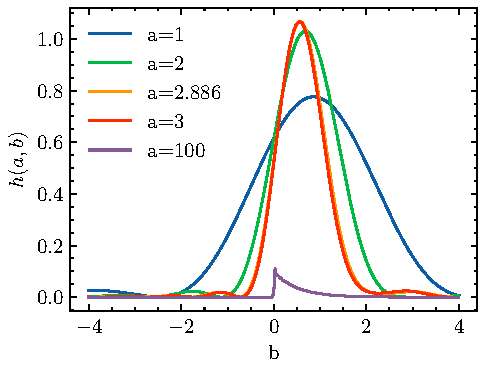
\includegraphics[width=\textwidth]{./img/bk-factor.pdf}
\end{subfigure}
\hspace{0.2cm}
\begin{subfigure}[b]{0.48\textwidth}
	\small
	% This file was created with tikzplotlib v0.10.1.
\begin{tikzpicture}

\definecolor{darkgray176}{RGB}{176,176,176}

\begin{axis}[
colorbar,
colorbar style={ytick={0,0.2,0.4,0.6,0.8,1,1.2},yticklabels={
  \(\displaystyle {0.0}\),
  \(\displaystyle {0.2}\),
  \(\displaystyle {0.4}\),
  \(\displaystyle {0.6}\),
  \(\displaystyle {0.8}\),
  \(\displaystyle {1.0}\),
  \(\displaystyle {1.2}\)
},ylabel={}},
colormap={mymap}{[1pt]
 rgb(0pt)=(0.001462,0.000466,0.013866);
  rgb(1pt)=(0.002267,0.00127,0.01857);
  rgb(2pt)=(0.003299,0.002249,0.024239);
  rgb(3pt)=(0.004547,0.003392,0.030909);
  rgb(4pt)=(0.006006,0.004692,0.038558);
  rgb(5pt)=(0.007676,0.006136,0.046836);
  rgb(6pt)=(0.009561,0.007713,0.055143);
  rgb(7pt)=(0.011663,0.009417,0.06346);
  rgb(8pt)=(0.013995,0.011225,0.071862);
  rgb(9pt)=(0.016561,0.013136,0.080282);
  rgb(10pt)=(0.019373,0.015133,0.088767);
  rgb(11pt)=(0.022447,0.017199,0.097327);
  rgb(12pt)=(0.025793,0.019331,0.10593);
  rgb(13pt)=(0.029432,0.021503,0.114621);
  rgb(14pt)=(0.033385,0.023702,0.123397);
  rgb(15pt)=(0.037668,0.025921,0.132232);
  rgb(16pt)=(0.042253,0.028139,0.141141);
  rgb(17pt)=(0.046915,0.030324,0.150164);
  rgb(18pt)=(0.051644,0.032474,0.159254);
  rgb(19pt)=(0.056449,0.034569,0.168414);
  rgb(20pt)=(0.06134,0.03659,0.177642);
  rgb(21pt)=(0.066331,0.038504,0.186962);
  rgb(22pt)=(0.071429,0.040294,0.196354);
  rgb(23pt)=(0.076637,0.041905,0.205799);
  rgb(24pt)=(0.081962,0.043328,0.215289);
  rgb(25pt)=(0.087411,0.044556,0.224813);
  rgb(26pt)=(0.09299,0.045583,0.234358);
  rgb(27pt)=(0.098702,0.046402,0.243904);
  rgb(28pt)=(0.104551,0.047008,0.25343);
  rgb(29pt)=(0.110536,0.047399,0.262912);
  rgb(30pt)=(0.116656,0.047574,0.272321);
  rgb(31pt)=(0.122908,0.047536,0.281624);
  rgb(32pt)=(0.129285,0.047293,0.290788);
  rgb(33pt)=(0.135778,0.046856,0.299776);
  rgb(34pt)=(0.142378,0.046242,0.308553);
  rgb(35pt)=(0.149073,0.045468,0.317085);
  rgb(36pt)=(0.15585,0.044559,0.325338);
  rgb(37pt)=(0.162689,0.043554,0.333277);
  rgb(38pt)=(0.169575,0.042489,0.340874);
  rgb(39pt)=(0.176493,0.041402,0.348111);
  rgb(40pt)=(0.183429,0.040329,0.354971);
  rgb(41pt)=(0.190367,0.039309,0.361447);
  rgb(42pt)=(0.197297,0.0384,0.367535);
  rgb(43pt)=(0.204209,0.037632,0.373238);
  rgb(44pt)=(0.211095,0.03703,0.378563);
  rgb(45pt)=(0.217949,0.036615,0.383522);
  rgb(46pt)=(0.224763,0.036405,0.388129);
  rgb(47pt)=(0.231538,0.036405,0.3924);
  rgb(48pt)=(0.238273,0.036621,0.396353);
  rgb(49pt)=(0.244967,0.037055,0.400007);
  rgb(50pt)=(0.25162,0.037705,0.403378);
  rgb(51pt)=(0.258234,0.038571,0.406485);
  rgb(52pt)=(0.26481,0.039647,0.409345);
  rgb(53pt)=(0.271347,0.040922,0.411976);
  rgb(54pt)=(0.27785,0.042353,0.414392);
  rgb(55pt)=(0.284321,0.043933,0.416608);
  rgb(56pt)=(0.290763,0.045644,0.418637);
  rgb(57pt)=(0.297178,0.04747,0.420491);
  rgb(58pt)=(0.303568,0.049396,0.422182);
  rgb(59pt)=(0.309935,0.051407,0.423721);
  rgb(60pt)=(0.316282,0.05349,0.425116);
  rgb(61pt)=(0.32261,0.055634,0.426377);
  rgb(62pt)=(0.328921,0.057827,0.427511);
  rgb(63pt)=(0.335217,0.06006,0.428524);
  rgb(64pt)=(0.3415,0.062325,0.429425);
  rgb(65pt)=(0.347771,0.064616,0.430217);
  rgb(66pt)=(0.354032,0.066925,0.430906);
  rgb(67pt)=(0.360284,0.069247,0.431497);
  rgb(68pt)=(0.366529,0.071579,0.431994);
  rgb(69pt)=(0.372768,0.073915,0.4324);
  rgb(70pt)=(0.379001,0.076253,0.432719);
  rgb(71pt)=(0.385228,0.078591,0.432955);
  rgb(72pt)=(0.391453,0.080927,0.433109);
  rgb(73pt)=(0.397674,0.083257,0.433183);
  rgb(74pt)=(0.403894,0.08558,0.433179);
  rgb(75pt)=(0.410113,0.087896,0.433098);
  rgb(76pt)=(0.416331,0.090203,0.432943);
  rgb(77pt)=(0.422549,0.092501,0.432714);
  rgb(78pt)=(0.428768,0.09479,0.432412);
  rgb(79pt)=(0.434987,0.097069,0.432039);
  rgb(80pt)=(0.441207,0.099338,0.431594);
  rgb(81pt)=(0.447428,0.101597,0.43108);
  rgb(82pt)=(0.453651,0.103848,0.430498);
  rgb(83pt)=(0.459875,0.106089,0.429846);
  rgb(84pt)=(0.4661,0.108322,0.429125);
  rgb(85pt)=(0.472328,0.110547,0.428334);
  rgb(86pt)=(0.478558,0.112764,0.427475);
  rgb(87pt)=(0.484789,0.114974,0.426548);
  rgb(88pt)=(0.491022,0.117179,0.425552);
  rgb(89pt)=(0.497257,0.119379,0.424488);
  rgb(90pt)=(0.503493,0.121575,0.423356);
  rgb(91pt)=(0.50973,0.123769,0.422156);
  rgb(92pt)=(0.515967,0.12596,0.420887);
  rgb(93pt)=(0.522206,0.12815,0.419549);
  rgb(94pt)=(0.528444,0.130341,0.418142);
  rgb(95pt)=(0.534683,0.132534,0.416667);
  rgb(96pt)=(0.54092,0.134729,0.415123);
  rgb(97pt)=(0.547157,0.136929,0.413511);
  rgb(98pt)=(0.553392,0.139134,0.411829);
  rgb(99pt)=(0.559624,0.141346,0.410078);
  rgb(100pt)=(0.565854,0.143567,0.408258);
  rgb(101pt)=(0.572081,0.145797,0.406369);
  rgb(102pt)=(0.578304,0.148039,0.404411);
  rgb(103pt)=(0.584521,0.150294,0.402385);
  rgb(104pt)=(0.590734,0.152563,0.40029);
  rgb(105pt)=(0.59694,0.154848,0.398125);
  rgb(106pt)=(0.603139,0.157151,0.395891);
  rgb(107pt)=(0.60933,0.159474,0.393589);
  rgb(108pt)=(0.615513,0.161817,0.391219);
  rgb(109pt)=(0.621685,0.164184,0.388781);
  rgb(110pt)=(0.627847,0.166575,0.386276);
  rgb(111pt)=(0.633998,0.168992,0.383704);
  rgb(112pt)=(0.640135,0.171438,0.381065);
  rgb(113pt)=(0.64626,0.173914,0.378359);
  rgb(114pt)=(0.652369,0.176421,0.375586);
  rgb(115pt)=(0.658463,0.178962,0.372748);
  rgb(116pt)=(0.66454,0.181539,0.369846);
  rgb(117pt)=(0.670599,0.184153,0.366879);
  rgb(118pt)=(0.676638,0.186807,0.363849);
  rgb(119pt)=(0.682656,0.189501,0.360757);
  rgb(120pt)=(0.688653,0.192239,0.357603);
  rgb(121pt)=(0.694627,0.195021,0.354388);
  rgb(122pt)=(0.700576,0.197851,0.351113);
  rgb(123pt)=(0.7065,0.200728,0.347777);
  rgb(124pt)=(0.712396,0.203656,0.344383);
  rgb(125pt)=(0.718264,0.206636,0.340931);
  rgb(126pt)=(0.724103,0.20967,0.337424);
  rgb(127pt)=(0.729909,0.212759,0.333861);
  rgb(128pt)=(0.735683,0.215906,0.330245);
  rgb(129pt)=(0.741423,0.219112,0.326576);
  rgb(130pt)=(0.747127,0.222378,0.322856);
  rgb(131pt)=(0.752794,0.225706,0.319085);
  rgb(132pt)=(0.758422,0.229097,0.315266);
  rgb(133pt)=(0.76401,0.232554,0.311399);
  rgb(134pt)=(0.769556,0.236077,0.307485);
  rgb(135pt)=(0.775059,0.239667,0.303526);
  rgb(136pt)=(0.780517,0.243327,0.299523);
  rgb(137pt)=(0.785929,0.247056,0.295477);
  rgb(138pt)=(0.791293,0.250856,0.29139);
  rgb(139pt)=(0.796607,0.254728,0.287264);
  rgb(140pt)=(0.801871,0.258674,0.283099);
  rgb(141pt)=(0.807082,0.262692,0.278898);
  rgb(142pt)=(0.812239,0.266786,0.274661);
  rgb(143pt)=(0.817341,0.270954,0.27039);
  rgb(144pt)=(0.822386,0.275197,0.266085);
  rgb(145pt)=(0.827372,0.279517,0.26175);
  rgb(146pt)=(0.832299,0.283913,0.257383);
  rgb(147pt)=(0.837165,0.288385,0.252988);
  rgb(148pt)=(0.841969,0.292933,0.248564);
  rgb(149pt)=(0.846709,0.297559,0.244113);
  rgb(150pt)=(0.851384,0.30226,0.239636);
  rgb(151pt)=(0.855992,0.307038,0.235133);
  rgb(152pt)=(0.860533,0.311892,0.230606);
  rgb(153pt)=(0.865006,0.316822,0.226055);
  rgb(154pt)=(0.869409,0.321827,0.221482);
  rgb(155pt)=(0.873741,0.326906,0.216886);
  rgb(156pt)=(0.878001,0.33206,0.212268);
  rgb(157pt)=(0.882188,0.337287,0.207628);
  rgb(158pt)=(0.886302,0.342586,0.202968);
  rgb(159pt)=(0.890341,0.347957,0.198286);
  rgb(160pt)=(0.894305,0.353399,0.193584);
  rgb(161pt)=(0.898192,0.358911,0.18886);
  rgb(162pt)=(0.902003,0.364492,0.184116);
  rgb(163pt)=(0.905735,0.37014,0.17935);
  rgb(164pt)=(0.90939,0.375856,0.174563);
  rgb(165pt)=(0.912966,0.381636,0.169755);
  rgb(166pt)=(0.916462,0.387481,0.164924);
  rgb(167pt)=(0.919879,0.393389,0.16007);
  rgb(168pt)=(0.923215,0.399359,0.155193);
  rgb(169pt)=(0.92647,0.405389,0.150292);
  rgb(170pt)=(0.929644,0.411479,0.145367);
  rgb(171pt)=(0.932737,0.417627,0.140417);
  rgb(172pt)=(0.935747,0.423831,0.13544);
  rgb(173pt)=(0.938675,0.430091,0.130438);
  rgb(174pt)=(0.941521,0.436405,0.125409);
  rgb(175pt)=(0.944285,0.442772,0.120354);
  rgb(176pt)=(0.946965,0.449191,0.115272);
  rgb(177pt)=(0.949562,0.45566,0.110164);
  rgb(178pt)=(0.952075,0.462178,0.105031);
  rgb(179pt)=(0.954506,0.468744,0.099874);
  rgb(180pt)=(0.956852,0.475356,0.094695);
  rgb(181pt)=(0.959114,0.482014,0.089499);
  rgb(182pt)=(0.961293,0.488716,0.084289);
  rgb(183pt)=(0.963387,0.495462,0.079073);
  rgb(184pt)=(0.965397,0.502249,0.073859);
  rgb(185pt)=(0.967322,0.509078,0.068659);
  rgb(186pt)=(0.969163,0.515946,0.063488);
  rgb(187pt)=(0.970919,0.522853,0.058367);
  rgb(188pt)=(0.97259,0.529798,0.053324);
  rgb(189pt)=(0.974176,0.53678,0.048392);
  rgb(190pt)=(0.975677,0.543798,0.043618);
  rgb(191pt)=(0.977092,0.55085,0.03905);
  rgb(192pt)=(0.978422,0.557937,0.034931);
  rgb(193pt)=(0.979666,0.565057,0.031409);
  rgb(194pt)=(0.980824,0.572209,0.028508);
  rgb(195pt)=(0.981895,0.579392,0.02625);
  rgb(196pt)=(0.982881,0.586606,0.024661);
  rgb(197pt)=(0.983779,0.593849,0.02377);
  rgb(198pt)=(0.984591,0.601122,0.023606);
  rgb(199pt)=(0.985315,0.608422,0.024202);
  rgb(200pt)=(0.985952,0.61575,0.025592);
  rgb(201pt)=(0.986502,0.623105,0.027814);
  rgb(202pt)=(0.986964,0.630485,0.030908);
  rgb(203pt)=(0.987337,0.63789,0.034916);
  rgb(204pt)=(0.987622,0.64532,0.039886);
  rgb(205pt)=(0.987819,0.652773,0.045581);
  rgb(206pt)=(0.987926,0.66025,0.05175);
  rgb(207pt)=(0.987945,0.667748,0.058329);
  rgb(208pt)=(0.987874,0.675267,0.065257);
  rgb(209pt)=(0.987714,0.682807,0.072489);
  rgb(210pt)=(0.987464,0.690366,0.07999);
  rgb(211pt)=(0.987124,0.697944,0.087731);
  rgb(212pt)=(0.986694,0.70554,0.095694);
  rgb(213pt)=(0.986175,0.713153,0.103863);
  rgb(214pt)=(0.985566,0.720782,0.112229);
  rgb(215pt)=(0.984865,0.728427,0.120785);
  rgb(216pt)=(0.984075,0.736087,0.129527);
  rgb(217pt)=(0.983196,0.743758,0.138453);
  rgb(218pt)=(0.982228,0.751442,0.147565);
  rgb(219pt)=(0.981173,0.759135,0.156863);
  rgb(220pt)=(0.980032,0.766837,0.166353);
  rgb(221pt)=(0.978806,0.774545,0.176037);
  rgb(222pt)=(0.977497,0.782258,0.185923);
  rgb(223pt)=(0.976108,0.789974,0.196018);
  rgb(224pt)=(0.974638,0.797692,0.206332);
  rgb(225pt)=(0.973088,0.805409,0.216877);
  rgb(226pt)=(0.971468,0.813122,0.227658);
  rgb(227pt)=(0.969783,0.820825,0.238686);
  rgb(228pt)=(0.968041,0.828515,0.249972);
  rgb(229pt)=(0.966243,0.836191,0.261534);
  rgb(230pt)=(0.964394,0.843848,0.273391);
  rgb(231pt)=(0.962517,0.851476,0.285546);
  rgb(232pt)=(0.960626,0.859069,0.29801);
  rgb(233pt)=(0.95872,0.866624,0.31082);
  rgb(234pt)=(0.956834,0.874129,0.323974);
  rgb(235pt)=(0.954997,0.881569,0.337475);
  rgb(236pt)=(0.953215,0.888942,0.351369);
  rgb(237pt)=(0.951546,0.896226,0.365627);
  rgb(238pt)=(0.950018,0.903409,0.380271);
  rgb(239pt)=(0.948683,0.910473,0.395289);
  rgb(240pt)=(0.947594,0.917399,0.410665);
  rgb(241pt)=(0.946809,0.924168,0.426373);
  rgb(242pt)=(0.946392,0.930761,0.442367);
  rgb(243pt)=(0.946403,0.937159,0.458592);
  rgb(244pt)=(0.946903,0.943348,0.47497);
  rgb(245pt)=(0.947937,0.949318,0.491426);
  rgb(246pt)=(0.949545,0.955063,0.50786);
  rgb(247pt)=(0.95174,0.960587,0.524203);
  rgb(248pt)=(0.954529,0.965896,0.540361);
  rgb(249pt)=(0.957896,0.971003,0.556275);
  rgb(250pt)=(0.961812,0.975924,0.571925);
  rgb(251pt)=(0.966249,0.980678,0.587206);
  rgb(252pt)=(0.971162,0.985282,0.602154);
  rgb(253pt)=(0.976511,0.989753,0.61676);
  rgb(254pt)=(0.982257,0.994109,0.631017);
  rgb(255pt)=(0.988362,0.998364,0.644924)
},
point meta max=1.06749233213328,
point meta min=1.43780715113311e-12,
tick pos=both,
x grid style={darkgray176},
xlabel={\(\displaystyle a\)},
xmin=0.01, xmax=8,
xtick style={color=black},
xtick={0,2,4,6,8},
xticklabels={
  \(\displaystyle {0}\),
  \(\displaystyle {2}\),
  \(\displaystyle {4}\),
  \(\displaystyle {6}\),
  \(\displaystyle {8}\)
},
y grid style={darkgray176},
ylabel={\(\displaystyle b\)},
ymin=-4, ymax=4,
ytick style={color=black},
ytick={-4,-2,0,2,4},
yticklabels={
  \(\displaystyle {\ensuremath{-}4}\),
  \(\displaystyle {\ensuremath{-}2}\),
  \(\displaystyle {0}\),
  \(\displaystyle {2}\),
  \(\displaystyle {4}\)
}
]
\addplot graphics [includegraphics cmd=\pgfimage,xmin=0.01, xmax=8, ymin=-4, ymax=4] {bk-factor-cmap-001.png};
\end{axis}

\end{tikzpicture}

	%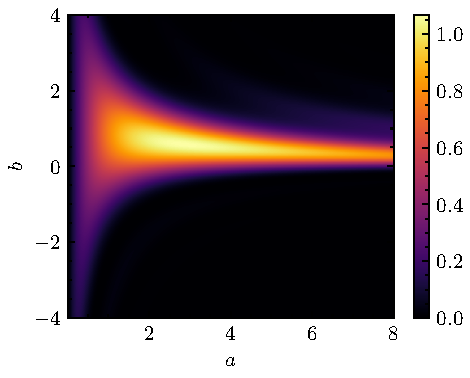
\includegraphics[width=\textwidth]{./img/bk-factor-cmap.pdf}
\end{subfigure}
\hspace{0.8cm}
\caption{Facteur de Boyd-Kleinman}
\label{fig:bk-factor}
\end{figure}


\section{Réalisation de la génération de seconde harmonique}

Le cristal doubleur choisi pour mon stage est un 

\begin{figure}[h]
	\centering
	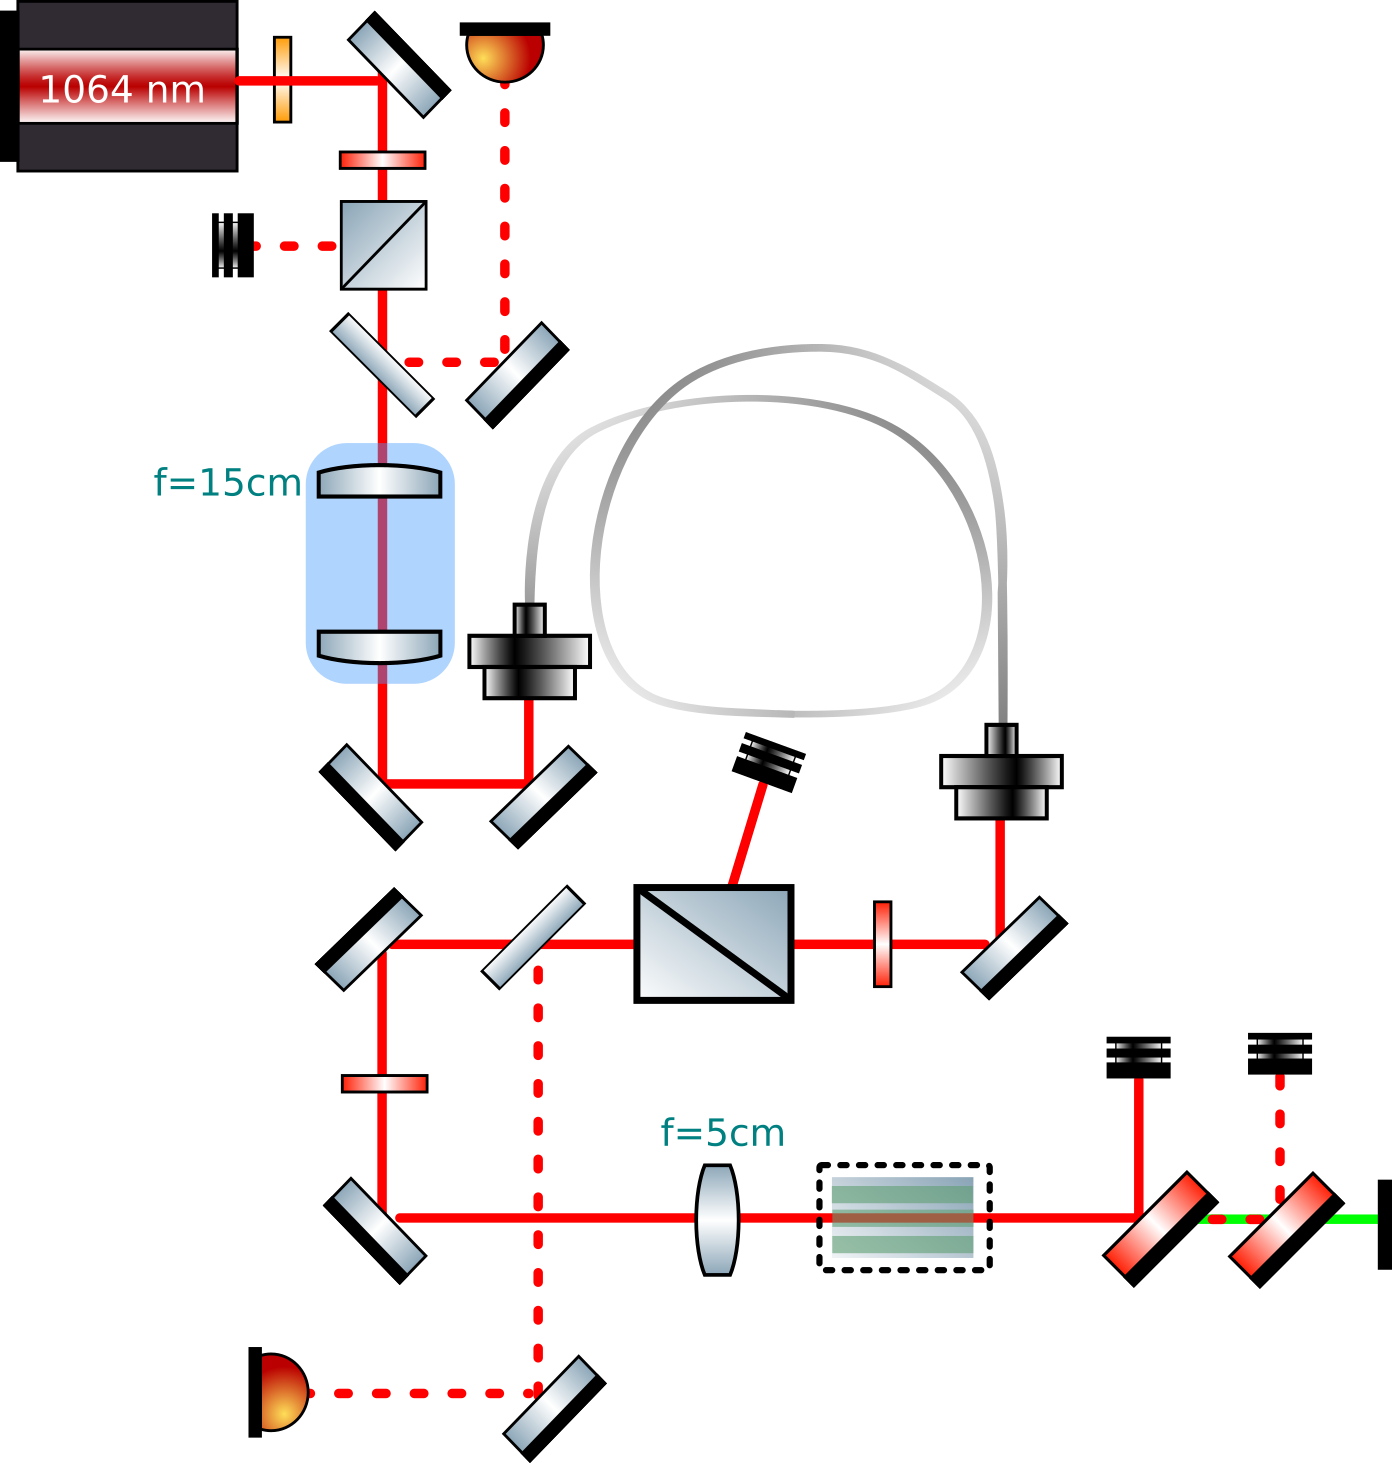
\includegraphics{./img/schema global.png}
	\caption{Schéma du montage global}
	\label{fig:global}
\end{figure}


Il faut noter que en pratique, on commence par choisir un waist et donc fixer un $a$, et on cherche ensuite à optimiser $b$ en ajustant la température et l'alignement.



\begin{figure}[h]
    \centering
    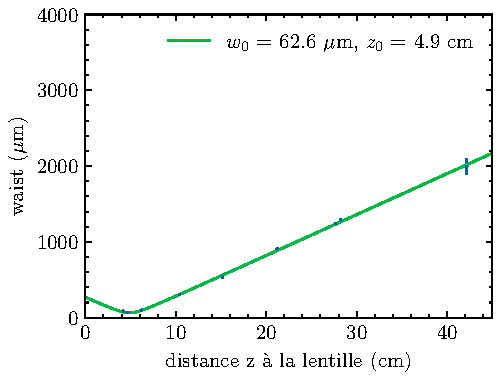
\includegraphics{../donnees/waist faisceau incident.pdf}
    \caption{Profil du faisceau incident sur le cristal}
\end{figure}

\begin{figure}[h]
    \centering
    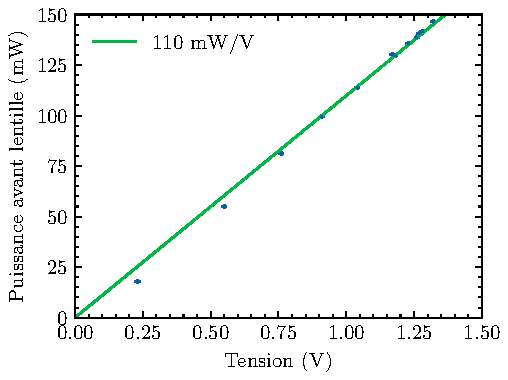
\includegraphics{../donnees/calib photodiode.pdf}
    \caption{Calibration de la photodiode (après glan)}
\end{figure}


\section{Étude à basse puissance}
Courbes basse puissance ($P2=f(P1^2)$ et $\alpha = f(T)$)

\begin{figure}[h]
    \centering
    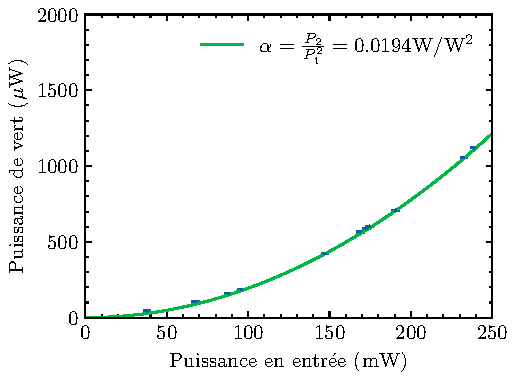
\includegraphics{../donnees/conversion basse puissance 82.5 C.pdf}
    \caption{Conversion à basse puissance à 82.5°C}
\end{figure}

\begin{figure}[h]
	\centering
	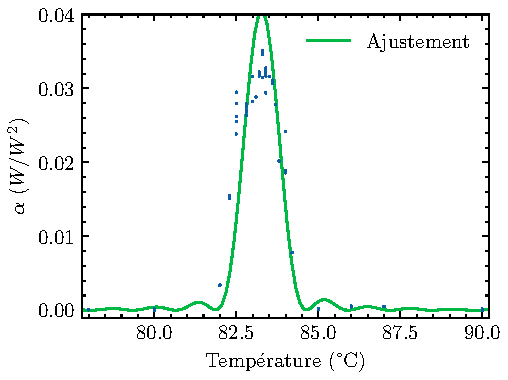
\includegraphics{./img/alpha bp.pdf}
	\caption{Dépendance en température de l'efficacité de conversion}
	\label{fig:alphabp}
\end{figure}

Discussion de l'hypothèse d'égalité des longueurs de Rayleigh

\begin{figure}[h]
	\centering
	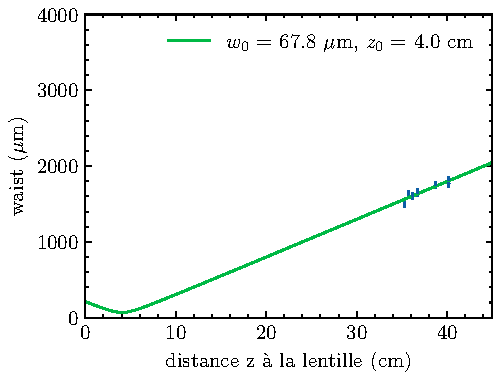
\includegraphics{./img/waist faisceau vert.pdf}
	\caption{Profil du faisceau vert généré}
	\label{fig:vert}
\end{figure}

\section{Étude à haute puissance}
\subsection{Caractérisation à haute puissance}
\subsection{Recherche d'un régime exploitable}
\section{Conclusion}

\appendix
\section{\'Equation d'onde non-linéaire}
\label{NL}
À partir des éqts de Maxwell, terme négligé (angle de double réfraction \cite{joffre}) \cite{boyd}

\section{Validité de l'hypothèse de non déplétion}
\label{ndepl}

\section{Efficacité de conversion dans un cristal périodiquement pôlé}
Étude par TF dans le plan (cf Dareaux)
%Dvpt en série de Fourier de d(z)
\label{BK}


\setcitestyle{numbers}
\bibliography{rapport.bib}
\bibliographystyle{unsrtnat}

\end{document}

